\chapter*{HEC 2016 : le corrigé}
  
%

\section*{EXERCICE} % HEC 2016

\noindent 
Soit $n$ et $p$ deux entiers supérieurs ou égaux à 1.
Si $M$ est une matrice de $\M{n,p},$ la matrice ${}^t{}M$ de 
$\M{p,n}$ désigne la transposée de $M.$\\
On identifie les ensembles $\M{1,1}$ et $\R$ en assimilant 
une matrice de $\M{1,1}$ à son unique coefficient.\\
On note $\B_n$ la base canonique de $\M{n,1}$ et 
$\B_p$ la base canonique de $\M{p,1}.$\\
Si $M \in \M{n,p}$ et $N \in \M{p,q}$ ($q 
\in \N^*$), {\it on admet} que 
${}^t{}{(MN)}={}^{t}{}{N}{}^{t}{}{M}$.

\begin{noliste}{1.}
 \setlength{\itemsep}{4mm}
 \item Soit $X$ une matrice colonne non nulle de 
 $\M{n,1}$ de composantes $x_1,x_2,...,x_n$ dans la base 
 $\B_n.$\\
 On pose : $A=X{}^{t}{}{X}$ et $\alpha = {}^{t}{}{X}X.$
 \begin{noliste}{a)}
  \setlength{\itemsep}{2mm}
  \item Exprimer $A$ et $\alpha$ en fonction de $x_1,x_2,...,x_n$.
  Justifier que la matrice $A$ est diagonalisable.
  
  \begin{proof}~
   \begin{noliste}{$\sbullet$}
    \item D'une part :
    \[
     A = X {}^t{}X =
     \begin{smatrix}
      x_1\\[.1cm]
      x_2\\[.1cm]
      \vdots \\[.1cm]
      x_n
     \end{smatrix}
     \times 
     \begin{smatrix}
      x_1 & x_2 & \cdots & x_n
     \end{smatrix}
     =
     \begin{smatrix}
      x_1^2 & x_1 x_2 & \cdots & x_1 x_n
      \\[.1cm]
      x_2 x_1 & x_2^2 & \cdots & x_2 x_n
      \\[.1cm]
      \vdots & \vdots & \ddots & \vdots 
      \\[.1cm]
      x_n x_1 & x_n x_2 & \cdots & x_n^2
     \end{smatrix}
    \]
    \conc{$A=
    \begin{smatrix}
     x_1^2 & x_1 x_2 & \cdots & x_1 x_n
     \\[.1cm]
     x_1 x_2 & x_2^2 & \cdots & x_2 x_n
     \\[.1cm]
     \vdots & \vdots & \ddots & \vdots 
     \\[.1cm]
     x_1 x_n & x_2 x_n & \cdots & x_n^2
    \end{smatrix}$}
     
    \item D'autre part :
    \[
     \alpha = {}^t{}X \, X =
      \begin{smatrix}
      x_1 & x_2 & \cdots & x_n
     \end{smatrix}
     \times
     \begin{smatrix}
      x_1\\
      x_2\\
      \vdots \\
      x_n
     \end{smatrix}
     = x_1^2 + x_2^2 + \cdots + x_n^2
    \]
    \conc{$\alpha = \Sum{k=1}{n} x_k^2$}
   \end{noliste}
   \conc{La matrice $A$ est une matrice symétrique réelle. Elle 
    est donc diagonalisable.}~\\[-1cm]
  \end{proof}


  \item Soit $f$ l'endomorphisme de $\M{n,1}$ de matrice $A$ dans la 
  base $\B_n.$\\
  Déterminer $\im(f)$ et $\kr(f)$ ; donner une base de 
  $\im(f)$ et préciser la dimension de $\kr(f)$.
  
  \begin{proof}~
   \begin{noliste}{$\sbullet$}
    \item D'après l'énoncé :
    \[
     \forall \, Y \in \M{n,1}, \ f(Y) = AY
    \]
    
    
    
    
    
    \newpage
    
    
    
    
    
    
    \item On note $\B_n=(e_1, \ldots, e_n)$. Donc :
    \[
     \forall i \in \llb 1, n\rrb, \ e_i = 
     \begin{smatrix}
      0\\
      \vdots \\
      0\\
      1\\
      0\\
      \vdots \\
      0
     \end{smatrix}
     \begin{sarray}{c}
      \\
      \\
      \text{$\eme{i}$ ligne} \\
      \\
      \\
     \end{sarray}
    \]
    \item Par caractérisation de l'image d'une application 
    linéaire :
    \[
     \im(f) = \Vect{f(e_1),f(e_2), \ldots, f(e_n)}
    \]
    Or, pour tout $i\in \llb 1,n \rrb$ :
    \[
     f(e_i)=A \times e_i = 
     \begin{smatrix}
      x_1 x_i\\[.1cm]
      x_2 x_i\\[.1cm]
      \vdots \\[.1cm]
      x_n x_i
     \end{smatrix}
     = x_i \cdot
     \begin{smatrix}
      x_1\\[.1cm]
      x_2\\[.1cm]
      \vdots \\[.1cm]
      x_n
     \end{smatrix}
     = x_i \cdot X
    \]
    Donc :
    \[
     \im(f) = \Vect{x_1 \cdot X, x_2 \cdot X, \ldots, x_n \cdot X}
    \]
    Deux cas se présentent alors :
    \begin{noliste}{$\stimes$}
      \item si : $\forall i \in \llb 1,n \rrb$, $x_i=0$, alors :
      $\im(f) = \Vect{0_{\M{n,1}}} = \{0_{\M{n,1}}\}$.
      \item si : $\exists i \in \llb 1,n \rrb$, $x_i \neq 0$, alors :
      $\im(f) = \Vect{X}$.
    \end{noliste}
    Or $X$ est un vecteur non nul de $\M{n,1}$. Donc il existe 
    $i\in \llb 1,n \rrb$ tel que : $x_i \neq 0$.
    \conc{On en déduit : $\im(f) = \Vect{X}$.}
    
    \item Donc la famille $(X)$ :
    \begin{noliste}{$\stimes$}
      \item engendre $\im(f)$ ;
      \item est une famille libre, car elle est constituée d'un unique 
      vecteur non nul.
    \end{noliste}
    \conc{Ainsi, $(X)$ est une base de $\im(f)$.}
    
    \item D'après le théorème du rang :
    \[
     \dim(\kr(f)) \ + \ \dim(\im(f)) \ = \ \dim(\M{n,1}) \ = \ n
    \]
    Or la famille $(X)$ est une base de $\im(f)$, donc :
    \[
     \dim(\im(f)) \ = \ \Card((X)) \ = \ 1
    \]
    \conc{Ainsi : $\dim(\kr(f))=n-1$.}
    
    \item Soit $Y\in \M{n,1}$. Alors il existe $(y_1, \ldots, y_n)
    \in \R^n$ tel que : $Y=
    \begin{smatrix}
     y_1\\
     \vdots \\
     y_n
    \end{smatrix}$.
    \[
     \begin{array}{rcl}
      Y \in \kr(f) & \Leftrightarrow & f(Y)=0_{\M{n,1}}
      \ \Leftrightarrow \ AY = 0_{\M{n,1}}
      \\[.2cm]
      & \Leftrightarrow & \left\{
      \begin{array}{rrrrrrrrrcl}
       x_1^2 \ y_1 & + & x_1 x_2 \ y_2 & + & x_1 x_3 \ y_3 & + & 
       \cdots & + & x_1 x_n \ y_n & = & 0
       \\[.1cm]
       x_1 x_2 \ y_1 & + & x_2^2 \ y_2 & + & x_2x_3 \ y_3 & + & 
       \cdots & + & x_2 x_n \ y_n & = & 0
       \\[.1cm]
       \vdots & & \vdots & & \vdots & & & & \vdots & & \vdots
       \\
       x_1 x_n \ y_1 & + & x_2 x_n \ y_2 & + & x_3 x_n \ y_3 & + & 
       \cdots & + & x_n^2 \ y_n & = & 0
      \end{array}
      \right.
     \end{array}
    \]
    
    
    
    
    \newpage
    
    
    On observe alors :
    \[
    \begin{array}{rcl}
      Y \in \kr(f) & \Leftrightarrow &
      \left\{
      \begin{array}{rrrrrrrrrcl}
       x_1(x_1 \ y_1 & + & x_2 \ y_2 & + & x_3 \ y_3 & + & 
       \cdots & + & x_n \ y_n) & = & 0
       \\[.1cm]
       x_2 (x_1 \ y_1 & + & x_2 \ y_2 & + & x_3 \ y_3 & + & 
       \cdots & + & x_n \ y_n) & = & 0
       \\[.1cm]
       \vdots & & \vdots & & \vdots & & & & \vdots & & \vdots
       \\
       x_n (x_1 \ y_1 & + & x_2 \ y_2 & + & x_3 \ y_3 & + & 
       \cdots & + & x_n \ y_n) & = & 0
      \end{array}
      \right.
     \end{array}
    \]

    Or, comme $X$ est un vecteur non nul, il existe $i_0\in 
    \llb 1,n \rrb$ tel que : $x_{i_0} \neq 0$.\\
    On effectue alors l'opération suivante :
    \[
      L_{i_0} \leftarrow \dfrac{1}{x_{i_0}} \, L_{i_0}
    \]
    La ligne $L_{i_0}$ devient donc :
    \[
      x_1 \, y_1 \ + \ x_2 \, y_2 \ + \ x_3 \, y_3 \ + \
      \cdots \ + \ x_n \, y_n \ = \ 0
    \]
    On effectue ensuite les opérations :
    \[
     \left\{
     \begin{array}{rcl}
      L_1 & \leftarrow & L_1 - x_1 \, L_{i_0}\\
      L_2 & \leftarrow & L_2 - x_2 \, L_{i_0}\\
      L_3 & \leftarrow & L_3 - x_3 \, L_{i_0}\\
       & \vdots & \\
      L_n & \leftarrow & L_n - x_n \, L_{i_0}
     \end{array}
     \right.
    \]
    On obtient alors :
    \[
     Y \in \kr(f) \ \Leftrightarrow \ 
     \left\{
      x_1 \, y_1 \ + \ x_2 \, y_2 \ + \ x_3 \, y_3 \ + \
      \cdots \ + \ x_n \, y_n \ = \ 0
      \right.
    \]
    \conc{$\kr(f) = \left\{ Y \in \M{n,1} \ \vert \
      x_1 \, y_1 \ + \ x_2 \, y_2 \ + \ x_3 \, y_3 \ + \
      \cdots \ + \ x_n \, y_n \ = \ 0 \right\}$}~\\[-1.4cm]
   \end{noliste}
  \end{proof}

  
  \item Calculer la matrice $AX$. \\
  Déterminer les valeurs propres de $A$ 
  ainsi que les sous-espaces propres associés.
  
  \begin{proof}~
   \begin{noliste}{$\sbullet$}
    \item On calcule :
    \[
     AX = 
     \begin{smatrix}
     x_1^2 & x_1 x_2 & \cdots & x_1 x_n
     \\[.2cm]
     x_1 x_2 & x_2^2 & \cdots & x_2 x_n
     \\[.2cm]
     \vdots & \vdots & \ddots & \vdots 
     \\[.2cm]
     x_1 x_n & x_2 x_n & \cdots & x_n^2
    \end{smatrix}
    \begin{smatrix}
      x_1\\[.2cm]
      x_2\\[.2cm]
      \vdots \\[.2cm]
      x_n
     \end{smatrix}
     =
     \begin{smatrix}
      x_1^3 + x_1 x_2^2 + \cdots + x_1 x_n^2
      \\[.2cm]
      x_2 x_1^2 + x_2^3 + \cdots + x_2 x_n^2
      \\[.2cm]
      \vdots 
      \\[.2cm]
      x_n x_1^2 + x_n x_2^2 + \cdots + x_n^3
     \end{smatrix}
     =
     \begin{smatrix}
      \alpha x_1\\[.2cm]
      \alpha x_2\\[.2cm]
      \vdots \\[.2cm]
      \alpha x_n
     \end{smatrix}
     = \alpha \cdot X
    \]
    \conc{$AX = \alpha \cdot X$}
    
    \item En résumé :
    \begin{noliste}{$\stimes$}
      \item $f(X)=AX=\alpha \cdot X$,
      \item $X \neq 0_{\M{n,1}}$.
    \end{noliste}
    Donc $X$ est un vecteur propre de $f$ associé à la valeur propre 
    $\alpha \neq 0$.
    \conc{Ainsi le sous-espace propre associé à $\alpha$ vérifie :\\
    $E_\alpha \supset \Vect{X}$.}
    
%     \item Montrons que $0$ et $\alpha$ sont les valeurs 
%     propres de $f$.\\
%     Pour cela, on introduit une base $(U_1, 
%     \ldots, U_{n-1})$ de $\kr(f)$ (car $\dim(\kr(f))=n-1$ d'après la 
%     question précédente). \\
%     La famille 
%     ${\cal F} = (U_1, \ldots, U_{n-1},X)$ est une base de 
%     $\M{n,1}$ car :
%     \begin{noliste}{$\stimes$}
%       \item la famille ${\cal F}$ est libre.\\
%       En effet, la famille ${\cal F}$ est la concaténation de 
%       familles libres de sous-espaces propres associés à des 
%       valeurs propres distinctes (on rappelle : $\alpha \neq 0$).
%       \item $\Card({\cal F}) = (n-1)+1=n = \dim(\M{n,1})$
%     \end{noliste}
%     \conc{On en déduit que ${\cal F}$ est une base de $\M{n,1}$.}
%     
%     \item De plus, ${\cal F}$ est une base de vecteurs propres de 
%     $f$. %
%     \conc{Ainsi les valeurs propres de $f$ sont $0$ et $\alpha$.}
%     
%     
%     
%     
    \newpage
    
    \item En notant $E_0=\kr(f)$ le sous-espace propre de $f$ 
    associé à la valeur propre $0$, on sait que :
    \begin{noliste}{$\stimes$}
      \item $0$ et $\alpha$ sont valeurs propres de $f$,
      \item $\dim(E_0)=n-1$ et $\dim(E_\alpha)\geq 1$.
    \end{noliste}
    Donc :
    \[
      \dim(E_0) \ + \ \dim(E_{\alpha}) \ \geq \ n
    \]
    De plus, $f$ est diagonalisable, donc : $\Sum{\lambda \in 
    \spc(f)}{} \dim(E_{\lambda}) \ = \ \dim(\M{n,1}) \ = \ n$.\\
    On en déduit que :
    \begin{noliste}{$\stimes$}
      \item l'endomorphisme $f$ n'admet pas d'autres valeurs 
      propres que $0$ et $\alpha$ \\
      (sinon : $\Sum{\lambda \in 
      \spc(f)}{} \dim(E_{\lambda}) >n$)
      \item $\dim(E_0) + \dim(E_\alpha)=n$.
    \end{noliste}
    \conc{L'endomorphisme $f$ admet exactement deux valeurs 
    propres : $0$ et $\alpha$.}
    
    \item D'après ce qui précède :
    \[
     \begin{array}{ccccc}
      \dim(E_0) & + & \dim(E_\alpha) & = & n
      \\
      \shortparallel 
      \\
      n-1
     \end{array}
    \]
    Donc $\dim(E_\alpha)=1$. On obtient alors :
    \begin{noliste}{$\stimes$}
      \item la famille $(X)$ est une famille libre de $E_\alpha$,
      \item $\Card((X))=1=\dim(E_\alpha)$.
    \end{noliste}
    Donc $(X)$ est une base de $E_\alpha$.
    \conc{Finalement : $E_0=\kr(f)$ et $E_\alpha=\Vect{X}$.}
   \end{noliste}
   
   \begin{remarkL}{0.95}
   \begin{noliste}{$\sbullet$}
    \item Comme ${\cal F}$ est une base de vecteurs propres de $f$, on 
    retrouve que $f$ est diagonalisable.\\ 
    On a même :
    \[
     \Mat_{\cal F}(f) =
     \begin{smatrix}
      0 & \cdots & 0 & 0
      \\[.1cm]
      \vdots & \ddots & \vdots & \vdots
      \\[.1cm]
      0 & \cdots & 0 & 0
      \\[.1cm]
      0 & \cdots & 0 & \alpha
     \end{smatrix}
    \]
    
    \item On pouvait également montrer que $0$ et $\alpha$ sont 
    les seules valeurs propres de $f$ en utilisant un polynôme
    annulateur de cet endomorphisme.\\
    Détaillons cette méthode.
    \begin{noliste}{$\stimes$}
      \item On remarque :
      \[
        A^2 \ = \ A \times A \ = \ X {}^t{}X \times X {}^t{}X \ = 
	\ X\times
        {}^t{}X \, X \times {}^t{}X \ = \ X \ \alpha \ {}^t{}X
        \ = \ \alpha \cdot X{}^t{}X \ = \ \alpha \cdot A
      \]
      Donc : $A^2-\alpha \cdot A=0_{\M{n}}$.\\
      D'où : $Q(X)=X^2-\alpha \, X=X(X-\alpha)$ est un polynôme
      annulateur de $A$.\\
      Ces racines sont $0$ et $\alpha$. Donc : $\spc(f)=
      \spc(A) \subset \{0,\alpha\}$.
      
      \item Comme on sait par ailleurs que $0$ et $\alpha$ sont 
      bien valeurs propres de $f$, on obtient :
      \[
        \spc(f) = \{0,\alpha\}
      \]
    \end{noliste}
    \end{noliste}
   \end{remarkL}~\\[-1.4cm]
  \end{proof}
 \end{noliste}
 
 
 
 
 \newpage
 
 
 
 
 \item On suppose que $n$ et $p$ vérifient $1 \leq p \leq n$.\\
 Soit $(V_1,V_2,...,V_p)$ une famille libre de $p$ vecteurs de 
 $\M{n,1}.$\\
 On note $V$ la matrice de $\M{n,p}$ dont les colonnes sont, dans cet 
 ordre, $V_1,V_2,...,V_p.$\\
 Soit $g$ l'application linéaire de $\M{p,1}$ dans $\M{n,1}$ de matrice 
 $V$ dans les bases $\B_p$ et $\B_n$.
 \begin{noliste}{a)}
  \setlength{\itemsep}{2mm}
  \item Justifier que le rang de $V$ est égal à $p$. Déterminer 
  $\kr(g)$.
  
  \begin{proof}~
   \begin{noliste}{$\sbullet$}
    \item On note ${\cal G} = \Vect{V_1, \ldots, V_p}$.
    \begin{noliste}{$\stimes$}
      \item La famille $(V_1, \ldots, V_p)$ engendre ${\cal G}$.
      \item La famille $(V_1, \ldots, V_p)$ est libre.
    \end{noliste} 
    
    Donc $(V_1, \ldots, V_p)$ est une base de ${\cal G}$.\\
    Ainsi : ~\\[-.6cm]
    \[
     \rg(V) = \dim(\Vect{V_1, \ldots , V_p}) = \dim({\cal G})
     = \Card((V_1, \ldots, V_p))= p
    \]
    \conc{Donc : $\rg(V)=p$}~\\[-1cm]
    
    \begin{remark}
      On pouvait aussi rédiger de la manière suivante.\\
      Le rang d'une matrice est la dimension du sous-espace
      engendré par ses vecteurs colonnes, ici $V_1, \ldots,
      V_p$.\\
      Or la famille $(V_1, \ldots, V_p)$ est libre. Donc :
      $\rg(V)=p$.
    \end{remark}~\\[-1.2cm]

    
    \item D'après le théorème du rang :
    \[
     \begin{array}{ccccc}
      \dim(\kr(g)) & + & \dim(\im(g)) & = & \dim(\M{p,1}) \ = \ p
      \\
       & & \shortparallel 
      \\
      p \ = \ \rg(V) & = & \rg(g)
     \end{array}
    \]
    Donc : $\dim(\kr(g)) = 0$.
    \conc{Ainsi : $\kr(g) = \{0_{\M{p,1}}\}$.}~\\[-1.6cm]
   \end{noliste}
  \end{proof}
  
  \item Soit $Y$ une matrice colonne de $\M{p,1}.$\\
  Montrer que l'on a $VY=0$ si et seulement si l'on a ${}^t{}VVY=0$.
  
  \begin{proof}~
   \begin{liste}{\quad}
    \item[$(\Rightarrow)$]
    Supposons : $VY=0_{\M{n,1}}$. Alors :
    \[
     {}^t{}VVY = {}^t{}V \times VY = {}^t{} V \times 0_{\M{n,1}}
     = 0_{\M{p,1}}
    \]
    
    \item[$(\Leftarrow)$]
    Supposons ${}^t{}VVY=0_{\M{p,1}}$. Alors : ${}^t{} Y {}^t{} V
    VY=0_{\R}$. \\[.1cm]
    Donc, en notant $Z=VY$, on obtient :
    \[
     {}^t{}ZZ= {}^t{}(VY)VY = {}^t{}Y {}^t{} VVY=0_{\R}
    \]~\\[-.4cm]
    Or $Z\in \M{n,1}$, donc il existe $(z_1, \ldots, z_n) \in \R^n$
    tel que : $Z=
    \begin{smatrix}
     z_1\\
     \vdots \\
     z_n
    \end{smatrix}$. D'où :~\\[-.4cm]
    \[
     \Sum{i=1}{n} z_i^2 = {}^t{}ZZ=0_{\R}
    \]
    Or, pour tout $i \in \llb 1, n\rrb$, $z_i^2 \geq 0$. Donc :
    \[
     \forall i \in \llb 1,n \rrb, \ z_i^2 =0 \quad \mbox{donc} 
     \quad z_i=0
    \]
    Ainsi : $Z=0_{\M{n,1}}$, c'est-à-dire : $VY=0_{\M{n,1}}$.
   \end{liste}
   \conc{$VY=0_{\M{n,1}}$ \ $\Leftrightarrow$ \
   ${}^t{}VVY=0_{\M{p,1}}$}~\\[-1cm]
  \end{proof}
  
  
  
  
  \newpage
  
  
  
  \item En déduire que la matrice ${}^t{}VV$ est inversible.
  
  \begin{proof}~\\
   On note $h$ l'endomorphisme de $\M{p,1}$ tel que : 
   $\Mat_{\B_p}(h)= {}^t{}VV$.
   \begin{noliste}{$\sbullet$}
    \item D'après la question précédente, pour toute 
    matrice colonne $Y \in \M{p,1}$ :
    \[
     g(Y)=VY=0_{\M{n,1}} \quad 
     \Leftrightarrow \quad h(Y)={}^t{}VVY=0_{\M{p,1}}
    \]
    Donc $\kr(g)=\kr(h)$.
    
    \item De plus, d'après la question \itbf{2.a)}, $\kr(g)=
    \{0_{\M{p,1}}\}$. Donc $\kr(h)=\{0_{\M{p,1}}\}$.\\
    D'où $h$ est injective.\\
    L'application $h$ est un endomorphisme injectif en 
    dimension finie. Donc $h$ est bijectif.
    \conc{Ainsi ${}^t{}VV$ est inversible.}~\\[-1.4cm]
   \end{noliste}
  \end{proof}
 \end{noliste}
\end{noliste}


\newpage


\section*{PROBLÈME} % HEC 2016
\noindent 
{\it On s'intéresse dans ce problème à quelques aspects 
mathématiques de la fonction de production d'une entreprise
qui produit un certain bien à une époque donnée, à partir de deux 
facteurs de production travail et capital.}\\
\textbf{Dans tout le problème :}
\begin{noliste}{$\sbullet$}
 \item {\it On note respectivement $x$ et $y$ les quantités de 
 travail et de capital requises pour produire une certaine quantité de 
 ce bien.}
 \item {\it On suppose que $x>0$ et $y>0.$ On pose 
 $\mathcal{D}=(\R_+^*)^2$ et pour tout $(x,y)\in \mathcal{D},$ 
 $z=\dfrac{x}{y}.$}
\end{noliste}
{\it La partie III est indépendante des parties I et II.}


\subsection*{Partie I : Fonction de production CES (Constant Elasticity 
of Substitution).}

\noindent
{\it Dans toute cette partie,} on note $c$ un réel vérifiant $0<c<1$ et 
$\theta$ un réel vérifiant $\theta < 1$ avec $\theta \neq 0.$\\
Soit $f$ la fonction définie sur $\mathcal{D},$ à valeurs dans 
$\R_+^*$, telle que :
\[
\forall (x,y)\in \mathcal{D},\quad 
f(x,y)=\left(c \, x^\theta+(1-c) \, y^\theta\right)^{\frac{1}{\theta}} 
\quad \text{({\it fonction de production CES})}
\]
\begin{noliste}{1.}
 \setlength{\itemsep}{4mm}
 \item {\it Exemple.} Dans cette question \textbf{uniquement,} on prend 
 $\theta=-1$ et $c=\dfrac{1}{2}$.
 \begin{noliste}{a)}
  \setlength{\itemsep}{2mm}
  \item Montrer que pour tout $(x,y) \in \mathcal{D},$ on a : $f(x,y) = 
  \dfrac{2xy}{x+y}$. Justifier que $f$ est de classe $\Cont{2}$ sur 
  $\mathcal{D}$ et calculer pour tout $(x,y) \in \mathcal{D},$ les 
  dérivées partielles $\dfn{f}{1}(x,y)$ et $\dfn{f}{2}(x,y)$.
  
  \begin{proof}~
   \begin{noliste}{$\sbullet$}
    \item Soit $(x,y) \in {\cal D}$.
    \[
     \begin{array}{rcl}
      f(x,y) &=& \left( \dfrac{1}{2} x^{-1} + \left(1-\dfrac{1}{2}
      \right) y^{-1}\right)^{\frac{1}{-1}}
      \\[.6cm]
      &=& \left( \dfrac{1}{2x} + \dfrac{1}{2y} \right)^{-1}
      \ = \ \left(\dfrac{y+x}{2xy}\right)^{-1}
      \\[.6cm]
      &=& \dfrac{2xy}{y+x}
     \end{array}
    \]
    \conc{$\forall (x,y) \in {\cal D}$, $f(x,y) = 
    \dfrac{2xy}{x+y}$}
    
    \item La fonction $f$ est de classe $\Cont{2}$ sur ${\cal D}$
    en tant que quotient de fonctions polynomiales (donc de 
    classe $\Cont{2}$ sur ${\cal D}$) dont le dénominateur ne 
    s'annule pas ($\forall (x,y) \in {\cal D}$, $x+y>0$).
    \conc{La fonction $f$ est de classe $\Cont{2}$ sur 
    ${\cal D}$.}
    
    \item Soit $(x,y) \in {\cal D}$.
    \[
     \dfn{f}{1}(x,y) \ = \ \dfrac{2y (\bcancel{x}+y) - 
     \bcancel{2xy}}{(x+y)^2} \ = \ \dfrac{2y^2}{(x+y)^2}
    \]
    De même :
    \[
     \dfn{f}{2}(x,y) \ = \ \dfrac{2x^2}{(x+y)^2}
    \]
    \conc{$\forall (x,y) \in {\cal D}$, \\[.1cm]
    $\dfn{f}{1}(x,y) = \dfrac{2y^2}{(x+y)^2}$ \quad et \quad
    $\dfn{f}{2}(x,y) = \dfrac{2x^2}{(x+y)^2}$}~\\[-1.2cm]
   \end{noliste}
  \end{proof}
  
  
  
  
  
  \newpage
  
  

  
  \item Soit $w$ et $U$ les fonctions définies sur $\R_+^*$ par :
  $\forall t > 0$, $w(t)=\dfrac{2t}{1+t}$ et $U(t)=w(t)-t \, w'(t).$\\
  Dresser le tableau de variation de la fonction $U$ sur $\R_+^*$ et 
  étudier la convexité de $U$ sur $\R_+^*$.
  
  \begin{proof}~
   \begin{noliste}{$\sbullet$}
    \item La fonction $w$ est bien dérivable sur $]0,+\infty[$
    en tant que quotient de fonctions dérivables sur $]0,+\infty[$
    dont le dénominateur ne s'annule pas
    ($\forall t \in \ ]0, +\infty[$, $1+t >0$).\\
    Soit $t>0$.
    \[
     w'(t) \ = \ \dfrac{2(1+\bcancel{t}) - \bcancel{2t}}{(1+t)^2}
     \ = \ \dfrac{2}{(1+t)^2}
    \]
    
    \item On en déduit : 
    \[
     U(t) \ = \ w(t) - t \, w'(t) \ = \ \dfrac{2t}{1+t} - 
     \dfrac{2t}{(1+t)^2}
     \ = \ \dfrac{2t(\bcancel{1}+t) - \bcancel{2t}}{(1+t)^2}
     \ = \ \dfrac{2t^2}{(1+t)^2}
    \]
    
    \item La fonction $U$ est de classe $\Cont{2}$ sur $]0,+\infty[$
    en tant que quotient de fonctions de classe $\Cont{2}$ sur 
    $]0,+\infty[$ dont le dénominateur ne s'annule pas
    ($\forall t \in \ ]0,+\infty[$, $(1+t)^2>0$).\\
    Soit $t>0$.
    \[
     U'(t) \ = \ \dfrac{4t(1+t)^2 - 4t^2(1+t)}{(1+t)^4}
     \ = \ \dfrac{(1+t)(4t(1+\bcancel{t}) - \bcancel{4t^2})}{(1+t)^4}
     \ = \ \dfrac{4t}{(1+t)^3}
    \]
    On en déduit : 
    \[
     \forall t >0, \ U'(t) = \dfrac{4t}{(1+t)^3} >0
    \]
    On obtient le tableau de variations suivant :
    
    \begin{center}
      \begin{tikzpicture}[scale=0.8, transform shape]
        \tkzTabInit[lgt=4,espcl=3] %
        { %
        $t$ /1, %
        Signe de $U'(t)$ /1, %
        Variations de $U$ /2
        } %
        {$0$, $+\infty$} %
        \tkzTabLine{ , + , } % 
        \tkzTabVar{-/$0$, +/$2$} %
      \end{tikzpicture}
     \end{center}
     
     Détaillons les éléments de ce tableau :
     \begin{noliste}{$\stimes$}
      \item Calculons $\dlim{t\to 0^+} U(t)$.
      \[
       \dlim{t\to 0^+} U(t) = \dfrac{2 \times 0^2}{(1+0)^2} = 0
      \]
      \item Calculons $\dlim{t\to +\infty} U(t)$.
      \[
       U(t) = \dfrac{2t^2}{(1+t)^2} \ \eq{t}{+\infty} \ 
       \dfrac{2 \bcancel{t^2}}{\bcancel{t^2}} = 2
      \]
      Donc : $\dlim{t\to +\infty} U(t)=2$.
     \end{noliste}
     
     
     \newpage
     

     \item Soit $t>0$.
     \[
      U''(t) \ = \ \dfrac{4(1+t)^3 - 12t(1+t)^2}{(1+t)^6}
      \ = \ \dfrac{(1+t)^2\left( 4(1+t) -12t\right)}{(1+t)^6}
      \ = \ \dfrac{4(1-2t)}{(1+t)^4}
     \]
     Donc :
     \[
      U''(t) \geq 0 \ \Leftrightarrow \ 1-2t \geq 0 
      \ \Leftrightarrow \ \dfrac{1}{2} \geq t
     \]
     Donc la fonction $U''$ s'annule et change de signe en 
     $\dfrac{1}{2}$.
     \conc{La fonction $U$ n'est ni convexe, ni concave.}
   \end{noliste}
   \begin{remark}
     Sa courbe représentative admet un point d'inflexion au point
     de coordonnées $\left(\dfrac{1}{2},\dfrac{2}{9}\right)$.
   \end{remark}~\\[-1.4cm]
 \end{proof}
  
  \item On rappelle que $z=\dfrac{x}{y}$. Montrer que pour tout $(x,y) 
  \in \mathcal{D}$, on a $f(x,y)=y \, w(z)$.
  
  \begin{proof}~\\
   Soit $(x,y) \in {\cal D}$. On a bien $z=\dfrac{x}{y} >0$.
   \[
    y \, w(z) \ = \ y \, \dfrac{2z}{1+z} \ = \ \bcancel{y} \, 
    \dfrac{2 \frac{x}{\bcancel{y}}}{1+\frac{x}{y}}
    \ = \ \dfrac{2x}{\frac{y+x}{y}} \ = \ \dfrac{2xy}{y+x} \ = \ f(x,y)
   \]
   \conc{$\forall (x,y) \in {\cal D}$, $f(x,y)=y w(z)$}~\\[-1cm]
  \end{proof}

  
  \item Vérifier pour tout $(x,y) \in \mathcal{D}$, les relations : 
  $\dfn{f}{1}(x,y)=w'(z)$ et $\dfn{f}{2}(x,y)=U(z)$.
  
  \begin{proof}~
   \begin{noliste}{$\sbullet$}
    \item Soit $(x,y) \in {\cal D}$.
    \[
     w'(z) \ = \ \dfrac{2}{(1+z)^2} \ = \ \dfrac{2}{\left(1 + 
     \frac{x}{y}\right)^2} \ = \ \dfrac{2}{\left(\frac{y+x}{y}\right)^2}
     \ = \ \dfrac{2}{\frac{(x+y)^2}{y^2}} \ = \ 
     \dfrac{2y^2}{(x+y)^2} \ = \ \dfn{f}{1}(x,y)
    \]
    \conc{$\forall (x,y) \in {\cal D}$, $\dfn{f}{1}(x,y) = w'(z)$}
    
    \item Soit $(x,y) \in {\cal D}$.
    \[
     U(z) \ = \ \dfrac{2z^2}{(1+z)^2} \ = \ \dfrac{2\left(\frac{x}{y}
     \right)^2}{\left(1+\frac{x}{y}\right)^2}
     \ = \ \dfrac{2\frac{x^2}{\bcancel{y^2}}}
     {\frac{(x+y)^2}{\bcancel{y^2}}} \ = \ \dfrac{2x^2}{(x+y)^2}
     \ = \ \dfn{f}{2}(x,y)
    \]
    \conc{$\forall (x,y) \in {\cal D}$, $\dfn{f}{2}(x,y) = U(z)$}
   \end{noliste}
  \end{proof}
 \end{noliste}
 
 
 
 
 
 \newpage
 
 
 
 

 \item 
 \begin{noliste}{a)}
  \setlength{\itemsep}{2mm}
  \item Montrer que pour tout $(x,y) \in \mathcal{D}$ et pour tout réel 
  $\lambda >0,$ on a : $f(\lambda x,\lambda y)=\lambda \, f(x,y)$.
  
  \begin{proof}~\\
   Soit $(x,y) \in {\cal D}$. Soit $\lambda >0$.
   \[
    \begin{array}{rcl}
     f(\lambda x, \lambda y) &=&
     \left( c(\lambda x)^\theta + (1-c) (\lambda y)^\theta\right)^{
     \frac{1}{\theta}}
     \\[.4cm]
     &=& \left(c \lambda^\theta x^\theta + (1-c) \lambda^\theta
     y^\theta\right)^{\frac{1}{\theta}}
     \\[.4cm]
     &=& \left( \lambda^\theta (c x^\theta + (1-c) y^\theta)\right)^{
     \frac{1}{\theta}}
     \\[.4cm]
     &=& \lambda^{\bcancel{\theta} \times \frac{1}{\bcancel{\theta}}}
     (c x^\theta + (1-c) y^\theta))^{\frac{1}{\theta}}
     \\[.4cm]
     &=& \lambda \, f(x,y)
    \end{array}
   \]
   \conc{$\forall (x,y) \in {\cal D}$, $\forall \lambda >0$, 
   $f(\lambda x, \lambda y) = \lambda \, f(x,y)$.}~\\[-1cm]
  \end{proof}

  
  \item Justifier que $f$ est de classe $\Cont{2}$ sur $\mathcal{D}$ 
  et, pour tout $(x,y) \in \mathcal{D}$, calculer $\dfn{f}{1}(x,y)$ et 
  $\dfn{f}{2}(x,y)$.
  
  \begin{proof}~
   \begin{noliste}{$\sbullet$}
    \item La fonction $(x,y) \mapsto x^\theta$ est de classe $\Cont{2}$
    sur ${\cal D}$ car elle est la composée $\psi_1 \circ g_1$ où :
    \begin{noliste}{$\stimes$}
      \item $g_1 : (x,y) \mapsto x$ est :
    \end{noliste}
      \begin{liste}{-}
	\item de classe $\Cont{2}$ sur 
        ${\cal D}$ en tant que fonction polynomiale,
	\item telle que $g_1({\cal D}) \subset \ ]0,+\infty[$.
      \end{liste}
    \begin{noliste}{$\stimes$}
      \item $\psi_1 : u \mapsto u^\theta$ est de classe $\Cont{2}$ sur 
      $]0,+\infty[$.
    \end{noliste}
    De même, la fonction $(x,y) \mapsto y^\theta$ est de classe 
    $\Cont{2}$ sur ${\cal D}$.\\
    Donc la fonction $(x,y) \mapsto c x^\theta + (1-c) y^\theta$
    est de classe $\Cont{2}$ sur ${\cal D}$ en tant que 
    combinaison linéaire de fonctions de classe $\Cont{2}$ sur 
    ${\cal D}$.\\
    D'où la fonction $f$ est de classe $\Cont{2}$ sur ${\cal D}$
    car elle est la composée $\psi_2 \circ g_2$ où :
    \begin{noliste}{$\stimes$}
      \item $h_1 : (x,y) \mapsto c x^\theta + (1-c) y^\theta$ est :
    \end{noliste}
    \begin{liste}{-}
      \item de classe $\Cont{2}$ sur ${\cal D}$,
      \item telle que : $h_1({\cal D}) \subset \ ]0,+\infty[$, car 
      $c>0$ et $1-c>0$.
    \end{liste}
    \begin{noliste}{$\stimes$}
      \item $h_2 : u \mapsto u^{\frac{1}{\theta}}$ est de classe 
      $\Cont{2}$ sur $]0,+\infty[$.
    \end{noliste}
    \conc{La fonction $f$ est de classe $\Cont{2}$ sur ${\cal D}$.}
    
    \begin{remark}
     On détaille ici assez précisément l'obtention du 
     caractère $\Cont{2}$ de $f$.\\
     Le détail d'une seule composée sur les deux 
     aurait sans doute permis d'obtenir tous les points.
    \end{remark}
    
    \item Soit $(x,y) \in {\cal D}$.
    \[
     \dfn{f}{1}(x,y) \ = \ \dfrac{1}{\bcancel{\theta}}
     \times c \bcancel{\theta} x^{\theta -1} \times 
     (c x^\theta + (1-c) y^\theta)^{\frac{1}{\theta} -1}
     \ = \ c x^{\theta-1} (c x^\theta + (1-c) 
     y^\theta)^{\frac{1}{\theta} -1}
    \]
    De même :
    \[
     \dfn{f}{2}(x,y) \ = \ \dfrac{1}{\bcancel{\theta}}
     \times (1-c) \bcancel{\theta} y^{\theta -1} \times 
     (c x^\theta + (1-c) y^\theta)^{\frac{1}{\theta} -1}
     \ = \ (1-c) y^{\theta-1} (c x^\theta + (1-c) 
     y^\theta)^{\frac{1}{\theta} -1}
    \]
    \conc{$\forall (x,y) \in {\cal D}$, 
    $\dfn{f}{1}(x,y) = c x^{\theta-1} (c x^\theta + (1-c) 
    y^\theta)^{\frac{1}{\theta} -1}$ \\[.1cm]
    \qquad \qquad \qquad \quad et 
    $\dfn{f}{2}(x,y) = (1-c) y^{\theta-1} (c x^\theta + (1-c) 
    y^\theta)^{\frac{1}{\theta} -1}$}~\\[-1.4cm]
   \end{noliste}
  \end{proof}
  
  
  
  
  \newpage
  
  

  
  \item Déterminer pour tout $y>0$ fixé, le signe et la monotonie de la 
  fonction $x \mapsto \partial_1(f)(x,y).$\\
  Déterminer pour tout $x>0$ fixé, le signe et la monotonie de 
  la fonction $y \mapsto \dfn{f}{2}(x,y)$.
  
  \begin{proof}~
   \begin{noliste}{$\sbullet$}
    \item Soit $(x,y) \in {\cal D}$. On a :
    \begin{noliste}{$\stimes$}
      \item $c>0$ et $1-c>0$ (car $0<c<1$),
      \item $x^{\theta-1}>0$ et $y^{\theta-1}>0$,
      \item $c x^\theta + (1-c) y^\theta >0$. Donc :
      $(c x^\theta + (1-c) y^\theta)^{\frac{1}{\theta}-1}>0$
    \end{noliste}
    \conc{Ainsi : $\forall (x,y) \in {\cal D}$, 
    $\dfn{f}{1}(x,y) >0$ et $\dfn{f}{2}(x,y)>0$.}
    
    \item Soit $(x,y) \in {\cal D}$.
    \[
     \begin{array}{rcl}
      \dfn{f}{1}(x,y) &=& 
      c x^{\theta-1} (c x^\theta + (1-c) y^\theta)^{
      \frac{1}{\theta} -1}
      \ = \ c \dfrac{1}{x^{1-\theta}} \left( (c x^\theta 
      +(1-c) y^\theta)^{\frac{1}{\theta}}\right)^{1-\theta}
      \\[.6cm]
      &=& c \left( \dfrac{(c x^\theta + (1-c) y^\theta)^{
      \frac{1}{\theta}}}{x}\right)^{1-\theta}
      \ = \ c \left(\left( \dfrac{c x^\theta + (1-c) y^\theta)}
      {x^\theta}\right)^{\frac{1}{\theta}}\right)^{1-\theta}
      \\[.6cm]
      &=& c \left(c + (1-c) \left(\dfrac{y}{x}\right)^\theta 
      \right)^{\frac{1}{\theta}-1}
     \end{array}
    \]
    Deux cas se présentent alors :
    \begin{noliste}{$\stimes$}
      \item \dashuline{si $\theta >0$}, alors $\dfrac{1}{\theta}
      -1 >0$, car $\theta<1$.
      Soit $(x_1,x_2)\in ]0,
      +\infty[^2$.
      \[
       \begin{array}{rcl@{\quad}>{\it}R{4.5cm}}
        & & x_1 < x_2 
        \\[.2cm]
        & \Leftrightarrow & \dfrac{1}{x_1} > 
        \dfrac{1}{x_2} 
        & (car $x \mapsto \dfrac{1}{x}$ est strictement
        décroissante sur $]0,+\infty[$)
        \nl
        \nl[-.2cm]
        & \Leftrightarrow & 
        \dfrac{y}{x_1} > \dfrac{y}{x_2}
        & (car $y>0$)
        \nl
        \nl[-.2cm]
        & \Leftrightarrow & 
        \left(\dfrac{y}{x_1}\right)^\theta > 
        \left(\dfrac{y}{x_2}\right)^\theta
        & (car, comme $\theta>0$, $x\mapsto x^\theta$ est strictement 
        croissante sur $]0,+\infty[$)
        \nl
        \nl[-.2cm]
        & \Leftrightarrow & 
        (1-c)\left(\dfrac{y}{x_1}\right)^\theta > 
        (1-c)\left(\dfrac{y}{x_2}\right)^\theta
        & (car $c<1$)
        \nl
        \nl[-.2cm]
        & \Leftrightarrow & 
        c + (1-c)\left(\dfrac{y}{x_1}\right)^\theta > 
        c + (1-c)\left(\dfrac{y}{x_2}\right)^\theta
        \\[.6cm]
        & \Leftrightarrow &
        \left(c + (1-c)\left(\dfrac{y}{x_1}\right)^\theta 
        \right)^{\frac{1}{\theta}-1}
        > 
        \left(c + (1-c)\left(\dfrac{y}{x_2}\right)^\theta
        \right)^{\frac{1}{\theta} -1}
        & (car, comme $\dfrac{1}{\theta}-1>0$, 
        $x\mapsto x^{\frac{1}{\theta}-1}$ est strictement 
        croissante sur $]0,+\infty[$)
        \nl
        \nl[-.2cm]
        & \Leftrightarrow & 
        c\left(c + (1-c)\left(\dfrac{y}{x_1}\right)^\theta 
        \right)^{\frac{1}{\theta}-1}
        > 
        c\left(c + (1-c)\left(\dfrac{y}{x_2}\right)^\theta
        \right)^{\frac{1}{\theta} -1}
        & (car $c>0$)
        \nl
        \nl[-.2cm]
        & \Leftrightarrow & 
        \dfn{f}{1}(x_1,y) > \dfn{f}{1}(x_2,y)
       \end{array}
      \]
      Donc $x\mapsto \dfn{f}{1}(x,y)$ est strictement 
      décroissante sur $]0,+\infty[$.
      
      
      
      
      
      \newpage
      
      
      
      
      \item \dashuline{si $\theta <0$}, alors on a :
      $\dfrac{1}{\theta} -1<0$.\\
      Avec un raisonnement analogue au précédent, on obtient 
      que la fonction $x \mapsto \dfn{f}{1}(x,y)$ est strictement 
      décroissante sur $]0,+\infty[$.
    \end{noliste}
    On prouverait de même que $y \mapsto 
    \dfn{f}{2}(x,y)$ est 
    strictement décroissante sur $]0,+\infty[$.
    \conc{Les fonctions $x\mapsto \dfn{f}{1}(x,y)$
    et $y \mapsto \dfn{f}{2}(x,y)$ \\[.1cm]
    sont strictement 
    décroissantes sur $]0,+\infty[$.}~\\[-1.2cm]
   \end{noliste}
  \end{proof}

 \end{noliste}
 
 \item Soit $G$ la fonction définie sur $\mathcal{D}$ par 
 $G(x,y)=\dfrac{\dfn{f}{1}(x,y)}{\dfn{f}{2}(x,y)}$ 
 ({\it taux marginal de substitution technique}) et $g$ la fonction 
 définie sur $\R_+^*$ par : $\forall t>0$, 
 $g(t)=\dfrac{c}{1-c}t^{-1+\theta}$.
 \begin{noliste}{a)}
  \setlength{\itemsep}{2mm}
  \item Pour tout $(x,y) \in \mathcal{D}$, exprimer $G(x,y)$ en 
  fonction de $g(z)$.
  
  \begin{proof}~\\
   Soit $(x,y) \in {\cal D}$.
   \[
    \begin{array}{rcl}
     G(x,y) &=& \dfrac{\dfn{f}{1}(x,y)}{\dfn{f}{2}(x,y)}
     \\[.6cm]
     &=& \dfrac{c x^{\theta-1} \bcancel{(c x^\theta + (1-c) y^\theta)^{
     \frac{1}{\theta}-1}}}{(1-c) y^{\theta-1}\bcancel{(c x^\theta + 
     (1-c) y^\theta)^{\frac{1}{\theta}-1}}}
     \\[.6cm]
     &=& \dfrac{c}{1-c} \dfrac{x^{\theta-1}}{y^{\theta-1}}
     \ = \ \dfrac{c}{1-c} \left(\dfrac{x}{y}\right)^{\theta-1}
     \\[.6cm]
     &=& \dfrac{c}{1-c} z^{\theta-1}
     \ = \ \dfrac{c}{1-c} z^{-1+\theta}
     \ = \ g(z)
    \end{array}
   \]
   \conc{$\forall (x,y) \in {\cal D}$, $G(x,y)=g(z)$}~\\[-1cm]
  \end{proof}

  
  \item\label{3b} Pour tout $t>0,$ on pose $s(t)=-\dfrac{g(t)}{t 
  \, g'(t)}$.
  Calculer $s(z)$ ({\it élasticité de substitution}). Conclusion.
  
  \begin{proof}~
   \begin{noliste}{$\sbullet$}
    \item La fonction $g$ est dérivable sur $]0,+\infty[$ en tant
    qu'inverse d'une fonction dérivable sur $]0,+\infty[$ qui ne 
    s'annule pas
    ($\forall t>0$, $t^{1-\theta} >0$).\\
    Soit $t>0$.
    \[
     g'(t) \ = \ \dfrac{c}{1-c}(-1+\theta) t^{-2+\theta}
    \]
    
    \item Soit $(x,y)\in {\cal D}$. Alors $z=\dfrac{x}{y}>0$.
    \[
     s(z) \ = \ -\dfrac{g(z)}{zg'(z)} \ = \ 
     -\dfrac{\bcancel{\frac{c}{1-c}} \, z^{-1+\theta}}
     {z \, \bcancel{\frac{c}{1-c}} (-1+\theta) z^{-2+\theta}}
     \ = \ - \dfrac{\bcancel{z^{-1+\theta}}}
     {\bcancel{z^{-1+\theta}} (-1+\theta)}
     \ = \ \dfrac{1}{1-\theta}
    \]
    \conc{$\forall (x,y) \in {\cal D}$, $s(z) = \dfrac{1}{1-\theta}$}
    
    \conc{On en déduit que l'élasticité de substitution est 
    constante, égale à $\dfrac{1}{1-\theta}$. \\
    En particulier, elle ne 
    dépend pas de $z$.}~\\[-1.4cm]
   \end{noliste}
  \end{proof}
 \end{noliste}
 
 
 
 
 \newpage
 
 
 
 
 \item Soit $w$ et $U$ les fonctions définies sur $\R_+^*$ par :
 $\forall t>0,$ $w(t)=f(t,1)$ et $U(t)=w(t)-t \, w'(t)$.
 \begin{noliste}{a)}
  \setlength{\itemsep}{2mm}
  \item Montrer que pour tout $(x,y) \in \mathcal{D},$ on a : 
  $f(x,y)=y \, w(z)$.
  
  \begin{proof}~\\
   Soit $(x,y) \in {\cal D}$.
   \[
    \begin{array}{rcl}
     y \, w(z) &=& y \, f(z,1) 
     \ = \ y (cz^\theta + (1-c) 1^\theta)^{\frac{1}{\theta}}
     \\[.2cm]
     &=& y\left( c \left(\dfrac{x}{y}\right)^\theta +
     1-c\right)^{\frac{1}{\theta}}
     \ = \ y\left( c \, \dfrac{x^\theta}{y^\theta} +
     1-c\right)^{\frac{1}{\theta}}
     \\[.4cm]
     &=& (y^\theta)^{\frac{1}{\theta}} \left( c \, 
     \dfrac{x^\theta}{y^\theta} +
     1-c\right)^{\frac{1}{\theta}}
     \ = \ \left( y^\theta \left( c \, \dfrac{x^\theta}{y^\theta} +
     1-c\right)\right)^{\frac{1}{\theta}}
     \\[.4cm]
     &=& \left( c \, \bcancel{y^\theta}
     \dfrac{x^\theta}{\bcancel{y^\theta}} +
     (1-c) y^\theta \right)^{\frac{1}{\theta}}
     \ = \ (cx^\theta + (1-c)y^\theta)^{\frac{1}{\theta}}
     \\[.4cm]
     &=& f(x,y)
    \end{array}
   \]
   \conc{$\forall (x,y) \in {\cal D}$, $f(x,y)=y \, w(z)$}~\\[-1cm]
  \end{proof}

  
  \item En distinguant les deux cas $0 < \theta < 1$ et $\theta < 0$, 
  dresser le tableau de variation de $U$ sur $\R_+^*.$\\
  Préciser $\dlim{t \to 0^+} U(t)$, $\dlim{t \to + \infty} U(t)$ ainsi 
  que la convexité de $U$ sur $\R_+^*$.
  
  \begin{proof}~
   \begin{noliste}{$\sbullet$}
    \item La fonction $w$ est dérivable sur $]0,+\infty[$.\\
    Soit $t>0$.
    \[
     w'(t) \ = \ \dfrac{1}{\bcancel{\theta}} \times c \bcancel{\theta}
     t^{\theta-1} \times (c t^\theta + 1-c)^{\frac{1}{\theta}-1}
     \ = \ c t^{\theta -1} (c t^\theta + 1-c)^{\frac{1}{\theta}-1}
    \]
    
    \item On obtient alors :
    \[
     \begin{array}{rcl}
      U(t) &=& w(t)- t \, w'(t)
      \\[.2cm]
      &=& (c t^\theta +1-c)^{\frac{1}{\theta}} - t \times 
      c t^{\theta-1}(c t^\theta +1-c)^{\frac{1}{\theta}-1}
      \\[.2cm]
      &=& (c t^\theta +1-c)^{\frac{1}{\theta}} -
      c t^{\theta}(c t^\theta +1-c)^{\frac{1}{\theta}-1}
      \\[.2cm]
      &=& (c t^\theta +1-c)^{\frac{1}{\theta}-1}
      \left((\bcancel{ct^\theta}+1-c) - \bcancel{ct^\theta}\right)
      \\[.2cm]
      &=& (1-c)(c t^\theta +1-c)^{\frac{1}{\theta}-1}
     \end{array}
    \]
    
    \item La fonction $U$ est de classe $\Cont{2}$ sur 
    $]0,+\infty[$.\\
    Soit $t>0$.
    \[
     \begin{array}{rcl}
      U'(t) &=& (1-c)\left(\dfrac{1}{\theta}-1\right)
      \times c \theta t^{\theta-1} \times (c t^\theta 
      +1-c)^{\frac{1}{\theta}-2}
      \\[.4cm]
      &=& (1-c) \times \dfrac{1-\theta}{\bcancel{\theta}} \times
      c \bcancel{\theta} t^{\theta-1} \times (c t^\theta 
      +1-c)^{\frac{1}{\theta}-2}
      \\[.4cm]
      &=& c(1-c) (1-\theta) t^{\theta-1} (c t^\theta 
      +1-c)^{\frac{1}{\theta}-2}
     \end{array}
    \]
    Or, on a :
    \begin{noliste}{$\stimes$}
      \item $c>0$ et $1-c>0$ (car $0<c<1$),
      \item $1-\theta>0$ (car $\theta<1$),
      \item $t^{\theta-1}>0$ (car $t>0$),
      \item $ct^\theta +1-c)>0$. Donc :
      $(ct^\theta +1-c)^{\frac{1}{\theta}-2}>0$
    \end{noliste}
    D'où : $U'(t)>0$.\\
    Ainsi, la fonction $U$ est strictement croissante sur 
    $]0,+\infty[$.
    
    
    
    \newpage
    
    
    
    \item Pour les calculs de limites, deux cas se présentent.
    \begin{noliste}{$\stimes$}
      \item \dashuline{Si $0<\theta<1$}, alors :
      $\dlim{t\to 0^+} t^\theta = 0$. \\
      De plus, par stricte 
      croissance de $x\mapsto \dfrac{1}{x}$ sur $]0,+\infty[$ :
      $
       \dfrac{1}{\theta} >1
      $.\\[.2cm]
      D'où :
      \[
       \dlim{t\to 0^+} U(t) \ = \ (1-c)(1-c)^{\frac{1}{\theta}-1}
       \ = \ (1-c)^{\frac{1}{\theta}}
      \]
      Par ailleurs : $\dlim{t\to +\infty} t^\theta = +\infty$. 
      Donc, comme $c>0$ :
      \[
       \dlim{t\to +\infty} (ct^\theta +1-c) \ = \ +\infty
      \]
      D'où, comme $\dfrac{1}{\theta}-1>0$ :
      \[
       \dlim{t\to +\infty} U(t) \ = \ +\infty
      \]
      On obtient alors le tableau de variations suivant :
      
      \begin{center}
      \begin{tikzpicture}[scale=0.8, transform shape]
        \tkzTabInit[lgt=4,espcl=3] %
        { %
        $t$ /1, %
        Signe de $U'(t)$ /1, %
        Variations de $U$ /2
        } %
        {$0$, $+\infty$} %
        \tkzTabLine{ , + , } % 
        \tkzTabVar{-/${\scriptstyle (1-c)^{\frac{1}{\theta}}}$, 
        +/$+\infty$} %
      \end{tikzpicture}
     \end{center}
     
     \item \dashuline{Si $\theta<0$}, alors :
      $\dlim{t\to 0^+} t^\theta = +\infty$. \\
      Donc, comme $c>0$ :
      \[
       \dlim{t\to 0^+} (ct^\theta +1-c) \ = \ +\infty
      \]
      De plus : $\dfrac{1}{\theta}<0$.
      D'où, comme $\dfrac{1}{\theta}-1<0$ :
      \[
       \dlim{t\to +\infty} U(t) \ = \ 0
      \]
      Par ailleurs : $\dlim{t\to +\infty} t^\theta = 0$. 
      Donc, comme $\dfrac{1}{\theta}-1<0$ :
      \[
       \dlim{t\to +\infty} U(t) \ = \ (1-c)(1-c)^{\frac{1}{\theta}-1}
       \ = \ (1-c)^{\frac{1}{\theta}}
      \]
      On obtient alors le tableau de variations suivant :
      
      \begin{center}
      \begin{tikzpicture}[scale=0.8, transform shape]
        \tkzTabInit[lgt=4,espcl=3] %
        { %
        $t$ /1, %
        Signe de $U'(t)$ /1, %
        Variations de $U$ /2
        } %
        {$0$, $+\infty$} %
        \tkzTabLine{ , + , } % 
        \tkzTabVar{-/$0$, 
        +/${\scriptstyle (1-c)^{\frac{1}{\theta}}}$} %
      \end{tikzpicture}
     \end{center}
     
     \begin{remark}
      On retrouve bien le cas $\theta=-1$ développé en question 
      \itbf{1.b)}.
     \end{remark}
    \end{noliste}
    
    
    
    
    \newpage
    
    
    
    \item Étudions l'éventuelle convexité de $U$.\\
    Soit $t>0$.
    \[
     \begin{array}{rcl}
      U''(t) &=& c(1-c)(1-\theta)(\theta-1)t^{\theta-2}
      (ct^\theta +1-c)^{\frac{1}{\theta}-2} 
      \\[.2cm]
      & & + \
      c(1-c)(1-\theta)t^{\theta-1} \left(\dfrac{1}{\theta}-2\right)
      \times c \theta t^{\theta-1} \times 
      (c t^\theta +1-c)^{\frac{1}{\theta}-3}
      \\[.4cm]
      &=& c(1-c)(1-\theta)t^{\theta-2}
      (c t^\theta +1-c)^{\frac{1}{\theta}-3}
      \left((\theta-1)(ct^\theta +1-c) + t^\theta 
      \, \dfrac{1-2\theta}{\bcancel{\theta}} \, c \bcancel{\theta}
      \right)
      \\[.4cm]
      &=& c(1-c)(1-\theta)t^{\theta-2}
      (c t^\theta +1-c)^{\frac{1}{\theta}-3}
      (c \theta t^\theta - \bcancel{c t^\theta} + (\theta-1)(1-c)
      + \bcancel{ct^\theta} -2c \theta t^\theta)
      \\[.2cm]
      &=& c(1-c)(1-\theta)t^{\theta-2}
      (c t^\theta +1-c)^{\frac{1}{\theta}-3}
      \left((\theta-1)(1-c) - c\theta t^\theta\right)
     \end{array}
    \]
    On a : $0<c<1$, $\theta <1$ et $t>0$. Donc :
    \[
     c(1-c)(1-\theta)t^{\theta-2}
      (c t^\theta +1-c)^{\frac{1}{\theta}-3} >0
    \]
    D'où :
    \[
       \begin{array}{rcl}
        U''(t) \leq 0 & \Leftrightarrow & 
        (\theta-1)(1-c) - c \, \theta \, t^\theta \leq 0
        \\[.2cm]
        & \Leftrightarrow & 
        (\theta-1)(1-c) \leq c \, \theta \, t^\theta
        \\[.2cm]
        & \Leftrightarrow & 
        \dfrac{(\theta-1)(1-c)}{c\theta} \leq t^\theta
        \quad (*)
       \end{array}
      \]
    Deux cas se présentent alors :
    \begin{noliste}{$\stimes$}
      \item \dashuline{si $0<\theta<1$}, alors : 
      $\theta-1<0$. Donc : 
      \[
       \dfrac{(\theta-1)(1-c)}{c \, \theta} \ < \ 0
      \]
      Or : $t>0$. Donc $t^\theta >0$.\\
      L'inégalité $(*)$ est donc vérifiée pour tout $t\in \ 
      ]0,+\infty[$.\\
      Donc : $\forall t \in \ ]0,+\infty[$, $U''(t)\leq 0$.
      \conc{Si $0<\theta<1$, alors la fonction $U$ est 
      concave sur $\R_+^*$.}
      
      \item \dashuline{si $\theta<0$}, alors :
      \[
       \dfrac{(\theta-1)(1-c)}{c \, \theta} \ > \ 0
      \]
      De plus : $\dfrac{1}{\theta}<0$. Donc, par stricte 
      décroissance de la fonction $x\mapsto x^{\frac{1}{\theta}}$
      sur $]0,+\infty[$ :
      \[
       U''(t) \leq 0 \ \Leftrightarrow \
       \left(\dfrac{(\theta-1)(1-c)}{c \, \theta} \right)^{
       \frac{1}{\theta}} \geq t
      \]
      \conc{Si $\theta<0$, la fonction $U$ n'est ni convexe, ni 
      concave.\\
      Elle admet un point d'inflexion d'abscisse 
      $\left(\dfrac{(\theta-1)(1-c)}{c\theta} \right)^{
       \frac{1}{\theta}}$.}~\\[-1.4cm]
    \end{noliste}
   \end{noliste}
  \end{proof}
 \end{noliste}
\end{noliste}





\newpage





\subsection*{Partie II : Caractérisation des fonctions de production à 
élasticité de substitution constante.}
\noindent 
{\it Dans toute cette partie,} on note $\Psi$ une fonction 
définie et de classe $\Cont{2}$ sur $\mathcal{D},$ à valeurs dans 
$\R_+^*$, vérifiant la condition $\Psi(1,1)=1$ et pour tout réel 
$\lambda > 0,$ la relation : $\Psi(\lambda x, \lambda y)=\lambda \,
\Psi(x,y)$.\\
De plus, on suppose que pour tout $y>0$ fixé, la fonction $x \mapsto 
\dfn{\Psi}{1}(x,y)$ est strictement positive et strictement 
décroissante et que pour tout $x>0$ fixé, la fonction $y \mapsto 
\dfn{\Psi}{2}(x,y)$ est également strictement positive et strictement 
décroissante.
\begin{noliste}{1.}
 \setlength{\itemsep}{4mm}
 \setcounter{enumi}{4}
 \item Soit $v$ la fonction définie sur $\R_+^*$ par : $\forall t > 0,$ 
 $v(t)=\Psi(t,1).$
 \begin{noliste}{a)}
  \setlength{\itemsep}{2mm}
  \item Justifier que la fonction $v$ est de classe $\Cont{2}$, 
  strictement croissante et concave sur $\R_+^*$.
  
  \begin{proof}~
   \begin{noliste}{$\sbullet$}
    \item La fonction $\Psi$ est de classe $\Cont{2}$ sur ${\cal D}$.
    \conc{Donc la fonction $v$ est de classe $\Cont{2}$ sur 
    $]0,+\infty[$.}
    
    \item Soit $y>0$.\\
    Par définition de la dérivée partielle première $\dfn{\Psi}{1}$
    de $\Psi$, la fonction $x\mapsto \Psi(x,y)$ est dérivable sur
    $]0,+\infty[$ (car $\Psi$ est de classe $\Cont{1}$ sur 
    ${\cal D}$) de dérivée $x \mapsto \dfn{\Psi}{1}(x,y)$.\\
    Donc, en prenant $y=1$, on obtient :
    \[
     \forall t >0, \ v'(t) = \dfn{\Psi}{1}(t,1)
    \]
    Or, d'après l'énoncé, la fonction $x\mapsto \dfn{\Psi}{1}
    (t,1)$ vérifie : $\forall x>0$, $\dfn{\Psi}{1}(t,1)>0$.\\
    Donc : $\forall t>0$, $v'(t)>0$.
    \conc{Ainsi, la fonction $v$ est strictement croissante sur 
    $]0,+\infty[$.}
    
    Toujours d'après l'énoncé, la fonction $x\mapsto \dfn{\Psi}{1}
    (x,1)$ est strictement décroissante.\\
    Donc la fonction $v'$ est strictement décroissante.
    \conc{Ainsi, la fonction $v$ est concave sur $]0,+\infty[$.}
   \end{noliste}
   
   \begin{remark}
    Pour déterminer $v'$, on aurait pu utiliser la définition de la
    dérivée d'une fonction (à l'aide du taux d'accroissement).\\
    Soit $t>0$.
    \[
     \begin{array}{rcl@{\quad}>{\it}R{5cm}}
      v'(t) &=& \dlim{h\to 0} \dfrac{v(t+h)-v(t)}{h} 
      \\[.4cm]
      &=& 
      \dlim{h\to 0} \dfrac{\Psi(t+h,1) -\Psi(t,1)}{h} 
      & (par définition de $v$)
      \nl
      \nl[-.2cm]
      &=& 
      \dfn{\Psi}{1}(t,1) & (par définition de la 
      dérivée partielle première $\dfn{\Psi}{1}$)
     \end{array}
    \]
   \end{remark}
   
   
   
   
   
   \newpage
   
   
   
   
   \begin{remark}
    La preuve faite ici du caractère $\Cont{2}$ de $v$ rapportait sans 
    doute la totalité des points de barème.
    Mais elle n'est en fait pas si évidente.\\
    Plus précisément, $v$ est de classe $\Cont{2}$ sur 
    ${\cal D}$ car elle est la composée $\Psi \circ h_1$ où :
    \begin{noliste}{$\stimes$}
      \item $h_1:t \mapsto (t,1)$ est :
      \begin{noliste}{-}
      \item de classe $\Cont{2}$ sur $]0,+\infty[$,
      \item telle que : $h_1(]0,+\infty[) = \ ]0,+\infty[ \ \times \{1\}
      \subset {\cal D}$.
      \end{noliste}
      \item $\Psi$ est de classe $\Cont{2}$ sur ${\cal D}$.
    \end{noliste}
    Cependant, les fonctions de $\R$ dans $\R^2$, telles que :
    \[
    h_1:
    \begin{array}[t]{ccc}
     ]0,+\infty[ & \to & \R^2\\
     t & \mapsto & (t,1)
    \end{array}
    \]
    ne sont pas étudiées en ECE.\\
    Pour rédiger une preuve complète du caractère $\Cont{2}$ de $v$
    en restant dans le cadre du programme ECE, on aurait pu rédiger de 
    la manière suivante :
    \begin{noliste}{$\sbullet$}
      \item la fonction $\Psi$ est de classe $\Cont{2}$ sur ${\cal D}$,
      donc, par définition de la dérivée partielle première 
      $\dfn{\Psi}{1}$, la fonction $v$ est dérivable sur $]0,+\infty[$
      de dérivée $v'$ définie par :
      \[
       \forall t>0, \ v'(t) = \dfn{\Psi}{1}(t,1)
      \]
      
      \item De même, par définition de la dérivée partielle 
      seconde $\ddfn{\Psi}{1,1}$, la fonction $v'$ est dérivable
      sur $]0,+\infty[$ de dérivée $v''$ définie par :
      \[
       \forall t>0, \ v''(t) = \ddfn{\Psi}{1,1}(t,1)
      \]
      
      \item Il reste à montrer que la fonction $v''$ est 
      continue sur $]0,+\infty[$. Pour cela, on utilise la 
      définition de la continuité.
      On note $d$ la distance euclidienne sur $\R^2$.\\
      La fonction $\ddfn{\Psi}{1,1}$ est continue sur ${\cal D}$.\\
      Soit $(x_0,y_0)\in {\cal D}$. On a alors :
      $\forall \eps >0, \ \exists \eta >0, \ \forall (x,y) \in 
       {\cal D}$,
      \[
        d((x_0,y_0),(x,y)) < \eta \ \ \Rightarrow \ \
       \vert \ddfn{\Psi}{1,1}(x,y) - \ddfn{\Psi}{1,1}(x_0,y_0) \vert
       < \eps
      \]
      Soit $t_0>0$.\\
      En choisissant $x_0=t_0$ et $y_0=1$, on obtient alors :
      $\forall \eps >0, \ \exists \eta >0, \ \forall t \in 
       \ ]0,+\infty[$,
      \[
        d((t_0,1),(t,1)) < \eta \ \ \Rightarrow \ \
       \vert \ddfn{\Psi}{1,1}(t,1) - \ddfn{\Psi}{1,1}(t_0,1) \vert
       < \eps
      \]
      Or, par définition de la distance euclidienne sur $\R^2$ :
      \[
       d((t_0,1),(t,1)) \ = \ \sqrt{(t-t_0)^2 + (1-1)^2}
       \ = \ \sqrt{(t-t_0)^2} \ = \ \vert t-t_0 \vert
      \]
      Donc :
      $\forall \eps >0, \ \exists \eta >0, \ \forall t \in 
       \ ]0,+\infty[$,
      \[
        \vert t - t_0 \vert < \eta \ \Rightarrow \
       \vert v''(t) - v''(t_0) \vert
       < \eps
      \]
      C'est la définition de la continuité de $v''$ en $t_0$.\\
      La fonction $v''$ est continue en tout point $t_0$ de 
      $]0,+\infty[$. Donc la fonction $v''$ est continue 
      sur $]0,+\infty[$.\\
      On en déduit que $v$ est de classe $\Cont{2}$ sur 
      $]0,+\infty[$.
    \end{noliste}
   \end{remark}~\\[-1.4cm]
  \end{proof}

  
  
  
  \newpage
  
  
  
  
  \item Soit $\varphi$ la fonction définie sur $\R_+^*$ par : $\forall 
  t >0$, $\varphi(t)=v(t)-t \, v'(t)$. On suppose l'existence de la 
  limite de $\varphi(t)$ lorsque $t$ tend vers 0 par valeurs supérieures
  et que $\dlim{t \to 0^+} \varphi(t)=\mu$, avec $\mu \geq 0$.\\
  Déterminer pour tout $t>0,$ le signe de $\varphi(t)$ et montrer que 
  $\mu \leq 1$.
  
  \begin{proof}~
   \begin{noliste}{$\sbullet$}
    \item D'après la question précédente, la fonction $\varphi$
    est de classe $\Cont{1}$ sur $]0,+\infty[$ en tant que somme
    de fonctions de classe $\Cont{1}$ sur $]0,+\infty[$.\\
    Soit $t>0$.
    \[
     \varphi'(t) = \bcancel{v'(t)} - (\bcancel{1\times v'(t)}
     + t \, v''(t)) = -t v''(t)
    \]
    
    \item Or la fonction $v'$ est strictement décroissante
    sur $]0,+\infty[$, 
    donc : $v''(t)< 0$.\\
    D'où : $\varphi'(t) > 0$.\\
    On obtient le tableau de variations suivant :
    
    \begin{center}
      \begin{tikzpicture}[scale=0.8, transform shape]
        \tkzTabInit[lgt=4,espcl=3] %
        { %
        $t$ /1, %
        Signe de $\varphi'(t)$ /1, %
        Variations de $\varphi$ /2
        } %
        {$0$, $+\infty$} %
        \tkzTabLine{ , + , } % 
        \tkzTabVar{-/$\mu$, +/} %
      \end{tikzpicture}
     \end{center}
     
     \item Par stricte croissance de $\varphi$ sur $]0,+\infty[$ :
     \[
      \forall t>0, \ \varphi(t) > \mu \geq 0
     \]
     \conc{Ainsi : $\forall t>0$, $\varphi(t) > 0$.}
     
     \item Par ailleurs :
     \[
      \begin{array}{rcl@{\quad}>{\it}R{4cm}}
       \varphi(1) &=& v(1) - 1 \times v'(1)
       \ = \ \Psi(1,1) - v'(1)
       \\[.2cm]
       &=& 1- v'(1) & (d'après l'énoncé)
       \nl
       \nl[-.2cm]
       & < & 1 & (car, d'après \itbf{5.a)} : $\forall t>0$, 
       $v'(t)>0$)
      \end{array}
     \]
     Donc, par croissance de $\varphi$ sur $]0,+\infty[$ :
     \[
      \mu \leq \varphi(1) <1
     \]
     \conc{Ainsi : $\mu \leq 1$.}~\\[-1.4cm]
   \end{noliste}
  \end{proof}

  
  \item Montrer que : $\forall (x,y) \in \mathcal{D}$, 
  $\Psi(x,y)=y \, v(z)$.
  
  \begin{proof}~\\
   Soit $(x,y) \in {\cal D}$.
   \[
    \begin{array}{rcl@{\quad}>{\it}R{5.5cm}}
     y \, v(z) &=& y \, \Psi(z,1) \ = \ y \, \Psi\left(
     \dfrac{x}{y},1\right)
     \\[.4cm]
     &=& \Psi\left(\bcancel{y} \times \dfrac{x}{\bcancel{y}}, 
     y \times 1\right)
     & (car, d'après l'énoncé :\\ $\forall \lambda >0$, 
     $\lambda \Psi(x,y) = \Psi(\lambda x, \lambda y)$)
     \nl
     \nl[-.2cm]
     &=& \Psi(x,y)
    \end{array}
   \]
   \conc{$\forall (x,y) \in {\cal D}$, $\Psi(x,y) = y \, v(z)$}~\\[-1cm]
  \end{proof}
 \end{noliste}
 
 
 
 
 
 \newpage
 
 
 
 
 \item\label{6} 
 \begin{noliste}{a)}
  \setlength{\itemsep}{2mm}
  \item Pour tout $t>0,$ on pose : $h(t)=\dfrac{v'(t)}{\varphi(t)}$.\\
  Montrer que pour tout $(x,y) \in \mathcal{D},$ on a : 
  $\dfrac{\dfn{\Psi}{1}(x,y)}{\dfn{\Psi}{2}(x,y)}=h(z)$.
  
  \begin{proof}~
   \begin{noliste}{$\sbullet$}
    \item D'après la question précédente :
    \[
     \forall (x,y) \in {\cal D}, \ \Psi(x,y) = y \, v(z)
     = y \, v\Big(\frac{x}{y}\Big)
    \]
    
    \item En dérivant cette égalité par rapport à $x$, on obtient :
    $\forall (x,y) \in {\cal D}$,
    \[
     \dfn{\Psi}{1}(x,y) \ = \ \bcancel{y} \times \dfrac{1}{\bcancel{y}}
     v'(\frac{x}{y}) \ = \ v'(z)
    \]
    
    \item En dérivant par rapport à $y$, on obtient :
    $\forall (x,y) \in {\cal D}$,
    \[
     \dfn{\Psi}{2}(x,y) \ = \ v\Big(\frac{x}{y}\Big) + \bcancel{y} 
     \times \left( -
     \dfrac{x}{y^{\bcancel{2}}}\right) \times v'(\frac{x}{y})
     \ = \ v(z) - \dfrac{x}{y} \, v'(z) \ = \ v(z) - z \, v'(z)
    \]
    
    \item Soit $(x,y) \in {\cal D}$. On obtient alors :
    \[
     h(z) \ = \ \dfrac{v'(z)}{\varphi(z)}
     \ = \ \dfrac{v'(z)}{v(z) - z \, v'(z)}
     \ = \ \dfrac{\dfn{\Psi}{1}(x,y)}{\dfn{\Psi}{2}(x,y)}
    \]
   \end{noliste}
   \conc{$\forall (x,y) \in {\cal D}$, $h(z) =
   \dfrac{\dfn{\Psi}{1}(x,y)}{\dfn{\Psi}{2}(x,y)}$}~\\[-1cm]
  \end{proof}

  
  \item Pour tout $t>0,$ on pose : $\sigma(t)=-\dfrac{h(t)}{t \, 
  h'(t)}$. Déterminer pour tout $t>0,$ le signe de $\sigma(t)$.
  
  \begin{proof}~
   \begin{noliste}{$\sbullet$}
    \item La fonction $h$ est de classe $\Cont{1}$ sur 
    $]0,+\infty[$ en tant que quotient de fonctions de classe 
    $\Cont{1}$ sur $]0,+\infty[$, dont le dénominateur ne s'annule
    pas
    ($\forall t>0$, $\varphi(t) >0$, d'après la question 
    \itbf{5.b)}).\\
    Soit $t>0$.
    \[
     \begin{array}{rcl}
      h'(t) &=& \dfrac{v''(t) \varphi(t) - v'(t) \varphi'(t)}
      {(\varphi(t))^2}
      \\[.6cm]
      &=& \dfrac{v''(t) (v(t) - t \, v'(t)) 
      - v'(t) (-t \, v''(t))}
      {(\varphi(t))^2}
      \\[.6cm]
      &=& \dfrac{v(t) \, v''(t) - \bcancel{t \, v'(t) \, v''(t)} 
      + \bcancel{t \, v'(t) \, v''(t)}}
      {(\varphi(t))^2}
      \\[.4cm]
      &=& \dfrac{v(t) \, v''(t)}{(\varphi(t))^2}
     \end{array}
    \]
    
    \item On obtient alors :
    \[
     \sigma(t) = - \dfrac{h(t)}{t\, h'(t)} = -
     \dfrac{\frac{v'(t)}{\bcancel{\varphi(t)}}}
     {t \, \frac{v(t) \, v''(t)}{(\varphi(t))^{\bcancel{2}}}}
     = - \dfrac{v'(t) \, \varphi(t)}
     {t \, v(t) \, v''(t)}
    \]

    \item D'après l'énoncé : $v(t) >0$.\\
    D'après la question \itbf{5.a)} : $v'(t)>0$.\\
    D'après la question \itbf{5.b)} : $v''(t)<0$ et
    $\varphi(t) >0$.
    \conc{Ainsi : $\forall t >0$, $\sigma(t) >0$.}~\\[-1.4cm]
   \end{noliste}
  \end{proof}
 \end{noliste}
 
 
 
 
 \newpage
 
 
 
 \item Les fonctions $\sigma$ et $h$ sont celles qui ont été définies 
 dans la question \itbf{6}. On suppose que la fonction $\sigma$ est 
 constante sur $\R_+^*$ ; on note $\sigma_0$ cette constante et on 
 suppose $\sigma_0 \neq 1$. On pose : $r=1-\dfrac{1}{\sigma_0}$.
 \begin{noliste}{a)}
  \setlength{\itemsep}{2mm}
  \item\label{7a} Pour tout $t>0,$ on pose $\ell(t)=t^{1-r}h(t)$.
  Calculer $\ell'(t)$ et en déduire que : $\forall t >0$, 
  $h(t)=h(1)t^{r-1}$.
  
  \begin{proof}~
   \begin{noliste}{$\sbullet$}
    \item La fonction $\ell$ est de classe $\Cont{1}$ sur $]0,+\infty[$
    en tant que produit de fonctions de classe $\Cont{1}$ sur 
    l'intervalle $]0,+\infty[$.\\
    Soit $t>0$.
    \[
     \ell'(t) \ = \ (1-r) t^{-r} h(t) + t^{1-r} h'(t)
    \]
    
    \item Or : $\sigma_0 \ = \ \sigma(t) \ = \ -\dfrac{h(t)}{t \, 
    h'(t)}$.\\
    Donc : $h'(t) \ = \ -\dfrac{h(t)}{\sigma_0 \, t}$
    
    \item De plus : $1-r \ = \ \bcancel{1} - \left(\bcancel{1}
    -\dfrac{1}{\sigma_0}\right) \ = \ \dfrac{1}{\sigma_0}$.\\
    Donc :
    \[
     \ell'(t) \ = \ \dfrac{1}{\sigma_0} \, t^{-r} \, h(t)
     + t^{1-r} \times \left(-\dfrac{h(t)}{\sigma_0 \, t}\right)
     \ = \ \dfrac{t^{-r}}{\sigma_0} \, h(t) - \dfrac{t^{-r}}{\sigma_0}
     \, h(t) \ = \ 0
    \]
    \conc{Ainsi : $\forall t >0$, $\ell'(t)=0$.}
    
    \item Donc $\ell$ est une fonction constante. Ainsi, 
    pour tout $t>0$ :
    \[
     \begin{array}{ccc}
      \ell(t) &=& \ell(1) \ = \ 1^{1-r} h(1) \ = \ h(1)
      \\
      \shortparallel
      \\[.1cm]
      t^{1-r} \, h(t)
     \end{array}
    \]
    \conc{D'où : $\forall t>0$, $h(t) = h(1) \, t^{r-1}$.}~\\[-1.4cm]
   \end{noliste}
  \end{proof}

  
  \item Par une méthode analogue à celle de la question \itbf{7a}, 
  établir la relation : 
  \[
  \forall t >0, \  
  v(t)=\left(\dfrac{1+h(1)t^r}{1+h(1)}\right)^{\frac{1}{r}}
  \]
  
  \begin{proof}~
   \begin{noliste}{$\sbullet$}
    \item Soit $t>0$.
    \[
     \begin{array}{rcl}
      v(t) = \left( \dfrac{1+h(1) t^r}{1+h(1)}\right)^{\frac{1}{r}}
      & \Leftrightarrow & (v(t))^r = 
      \dfrac{1+h(1) t^r}{1+h(1)}
      \\[.4cm]
      & \Leftrightarrow & \dfrac{(v(t))^r}{1+h(1) t^r}
      = \dfrac{1}{1+h(1)}
     \end{array}
    \]
    Prouver l'égalité demandée revient donc à montrer que la 
    fonction $w:t \mapsto
    \dfrac{(v(t))^r}{1+h(1) t^r}$ est constante sur 
    $]0,+\infty[$.
    
    \item La fonction $w$ est de classe $\Cont{1}$ sur $]0,+\infty[$
    en tant que quotient de fonctions de classe $\Cont{1}$ sur
    $]0,+\infty[$ dont le dénominateur ne s'annule pas
    ($\forall t>0$, $1+h(1) t^r >0$).\\
    
    
    
    
    \newpage
    
    
    
    Soit $t>0$.
    \[
     \begin{array}{rcl}
      w'(t) &=& \dfrac{rv'(t) (v(t))^{r-1} (1+h(1)t^r)
      - (v(t))^r \left(r h(1) t^{r-1}\right)}
      {(1+h(1) t^r)^2}
      \\[.6cm]
      &=& r(v(t))^{r-1}
      \dfrac{v'(t)(1+h(1) t^r) - v(t) h(1)t^{r-1}}
      {(1+h(1) t^r)^2}
      \\[.6cm]
      &=& r(v(t))^{r-1}
      \dfrac{v'(t) +h(1) t^{r-1}(t \, v'(t) - v(t))}
      {(1+h(1) t^r)^2}
      \\[.6cm]
      &=& r(v(t))^{r-1}
      \dfrac{v'(t) - h(1) t^{r-1} \varphi(t)}
      {(1+h(1) t^r)^2}
     \end{array}
    \]
    Or : $\dfrac{v'(t)}{\varphi(t)} \ = \ h(t) \ = \ h(1) t^{r-1}$.
    Donc : $v'(t) \ = \ h(1) t^{r-1} \varphi(t)$.
    D'où :
    \[
     w'(t) \ = \ 0
    \]
    On en déduit que la fonction $w$ est constante. Donc, pour 
    tout $t>0$ :
    \[
     \begin{array}{ccc}
      w(t) &=& w(1) \ = \ 
      \dfrac{(v(1))^r}{1+h(1)} \ = \ 
      \dfrac{1}{1+h(1)}
      \\[-.1cm]
      \shortparallel
      \\[.1cm]
      \dfrac{(v(t))^r}{1+h(1) t^r}
     \end{array}
    \]
    En effet, d'après l'énoncé :
    \[
     v(1) \ = \ \Psi(1,1) \ = \ 1
    \]
    \conc{$\forall t>0$, $v(t) = 
    \left( \dfrac{1+h(1) t^r}{1+h(1)}\right)^{\frac{1}{r}}$
    }~\\[-1.4cm]
   \end{noliste}
  \end{proof}

  
  \item\label{7c} En déduire l'existence d'une constante $a \in ]0,1[$ 
  telle que : $\forall (x,y) \in \mathcal{D}$, 
  $\Psi(x,y)=\left(ax^r+(1-a)y^r\right)^{\frac{1}{r}}$.
  
  \begin{proof}~\\
   Soit $(x,y) \in {\cal D}$.
   \[
    \begin{array}{rcl@{\quad}>{\it}R{5cm}}
     \Psi(x,y) &=& y \, v(z) & (d'après la question \itbf{5.c)})
     \nl
     \nl[-.2cm]
     &=& y \left( \dfrac{1+h(1) z^r}{1+h(1)}\right)^{\frac{1}{r}}
     \\[.4cm]
     &=& (y^r)^{\frac{1}{r}}
     \left( \dfrac{1+h(1) \left(\frac{x}{y}\right)^r}
     {1+h(1)}\right)^{\frac{1}{r}}
     \\[.6cm]
     &=& \left( y^r \, \dfrac{1+h(1) \frac{x^r}{y^r}}
     {1+h(1)} \right)^{\frac{1}{r}}
     \\[.6cm]
     &=& \left(\dfrac{1}{1+h(1)} \, y^r + 
     \dfrac{h(1)}{1+h(1)} \, x^r\right)^{\frac{1}{r}}
    \end{array}
   \]
   \conc{Donc, en posant $a= \dfrac{h(1)}{1+h(1)}$ :\\
   $\forall (x,y) \in {\cal D}$, $\Psi(x,y) =
   (ax^r + (1-a) y^r)^{\frac{1}{r}}$.}~\\[-1cm]
  \end{proof}
  
  
  
  
  \newpage
  
  
  

  
  \item Quelle conclusion peut-on tirer des résultats des questions 
  \itbf{3.b)} et \itbf{7.c)} ?
  
  \begin{proof}~
   \begin{noliste}{$\sbullet$}
    \item D'après la question \itbf{3.b)}, toute fonction de 
    production CES possède une élasticité de substitution constante.
    
    \item Réciproquement, d'après la question \itbf{7.c)}, toute
    fonction de production possédant une élasticité de 
    substitution constante est une fonction de production CES.
   \end{noliste}
   
   \conc{Une fonction de production est à élasticité constante
   si et seulement si\\
   c'est une fonction de production CES.}
   
   \begin{remark}
    Ce résultat justifie l'appellation des fonctions de production
    CES : Constant Elasticity of Substitution.
   \end{remark}~\\[-1.4cm]
  \end{proof}
 \end{noliste}
 
 \item Soit $a \in \ ]0,1[$. Pour tout $t>0,$ soit $S_t$ la fonction 
 définie sur $]-\infty,1[ \setminus \{0\}$ par : 
 $S_t(r)=(at^r+1-a)^{\frac{1}{r}}$.
 \begin{noliste}{a)}
  \setlength{\itemsep}{2mm}
  \item On pose $H_t(r)=\ln S_t(r)$. Calculer la limite de $S_t(r)$ 
  lorsque $r$ tend vers 0.
  
  \begin{proof}~
   \begin{noliste}{$\sbullet$}
    \item Soit $r\in \ ]-\infty,1[ \, \setminus \, \{0\}$.
    \[
     H_t(r) \ = \ \ln(S_t(r)) \ = \ \dfrac{1}{r} \ln(at^r +1-a)
     \ = \ \dfrac{1}{r} \ln(1+ a(t^r-1))
    \]
    
    \item Or : $\dlim{r\to 0} t^r=1$. Donc : 
    $\dlim{r\to 0} a(t^r-1)=0$. D'où :
    \[
     \ln(1+a(t^r-1)) \eq{r}{0} a(t^r-1)
    \]
    Ainsi :
    \[
     H_t(r) \eq{r}{0} a \, \dfrac{t^r-1}{r} = a \,
     \dfrac{\ee^{r \ln(t)}-1}{r}
    \]
    
    \item Or : $\dlim{r \to 0} r \, \ln(t) =0$. Donc :
    \[
     \ee^{r\ln(t)} -1 \eq{r}{0} r \, \ln(t)
    \]
    D'où :
    \[
     H_t(r) \eq{r}{0} a \, \dfrac{\bcancel{r} \ln(t)}
     {\bcancel{r}} = a \, \ln(t)
    \]
    Ainsi : $\dlim{r\to 0} H_t(r)=a \, \ln(t)$.\\[.2cm]
    De plus : $\forall r \in \ ]-\infty, 1[ \, \setminus \, \{0\}$,
    $S_t(r) = \exp(H_t(r))$.
    \conc{D'où : $\dlim{r\to 0} S_t(r) = \exp(a \, \ln(t))
    = t^a$.}~\\[-1.4cm]
   \end{noliste}
  \end{proof}
  
  
  
  
  \newpage
  
  
  

  
  \item Pour tout couple $(x,y) \in \mathcal{D}$ fixé, on pose : 
  $N_{(x,y)}(r) = y \, S_z(r)$ et $F(x,y)=\dlim{r \to 0} 
  N_{(x,y)}(r)$.\\
  Montrer que pour tout $(x,y) \in \mathcal{D},$ on a 
  $F(x,y)=x^a \, y^{1-a}$ ({\it fonction de production de 
  Cobb-Douglas}).
  
  \begin{proof}~\\
   Soit $(x,y) \in {\cal D}$.\\
   D'après la question précédente :
   \[
    F(x,y) \ = \ \dlim{r\to 0} y \, S_z(r) \ = \ y \, z^a
    \ = \ y \, \left(\dfrac{x}{y}\right)^a \ = \ y \, 
    \dfrac{x^a}{y^a} \ = \ x^a \, y^{1-a}
   \]
   \conc{$\forall (x,y) \in {\cal D}$, $F(x,y)=x^a \, 
   y^{1-a}$.}~\\[-1cm]
  \end{proof}
 \end{noliste}
\end{noliste}




\subsection*{Partie III : Estimation des paramètres d'une fonction de 
production de Cobb-Douglas.}
\noindent 
Soit $a$ un réel vérifiant $0 < a < 1$ et $B$ un réel 
strictement positif.\\
On suppose que la production totale $Q$ présente une composante 
déterministe et une composante aléatoire.
\begin{noliste}{$\sbullet$}
 \item La {\it composante déterministe} est une fonction de 
 production de type Cobb-Douglas, c'est-à-dire telle que :
 \[
  \forall (x,y) \in \mathcal{D},\quad f(x,y)=Bx^ay^{1-a}
 \]
 
 \item La {\it composante aléatoire} est une variable aléatoire de la 
 forme $\exp(R)$ où $R$ est une variable aléatoire suivant la loi 
 normale centrée, de variance $\sigma^2>0$.
 
 \item La {\it production totale} $Q$ est une variable aléatoire à 
 valeurs strictement positives telle que :
 \[
  Q=Bx^ay^{1-a} \exp(R)
 \]
\end{noliste}
On suppose que les variables aléatoires $Q$ et $R$ sont définies sur 
le même espace probabilisé $(\Omega,\A,\Prob)$.

\begin{remark}
 En général, la fonction de production de Cobb-Douglas est 
 exprimée à l'aide de \var :
 \[
  Q = B \, X^a \, Y^{1-a}
 \]
 où :
 \begin{noliste}{$\stimes$}
  \item la \var $X$ exprime la quantité de travail nécessaire à la
   production d'un volume physique de ce bien (par exemple pour $1$
   tonne, ou $1$ litre, ou encore un nombre fixé de produits),
  \item la \var $Y$ exprime la quantité de capital nécessaire à la
   production de la même quantité de ce bien de consommation.
 \end{noliste}
 Le sujet définit la fonction de production de Cobb-Douglas de
 manière un peu différente en mêlant réalisations et variables 
 aléatoires.\\
 On sera d'autant plus attentif à la nature des objets manipulés.
\end{remark}

\noindent
On pose : $b=\ln(B)$, $u=\ln(x) - \ln(y)$ et $T=\ln(Q)-\ln(y)$. On a 
donc : $T=au+b+R$.\\
On sélectionne $n$ entreprises ($n \geq 1$) qui produisent le bien 
considéré à l'époque donnée.\\
On mesure pour chaque entreprise $i$ ($i \in \llb 1,n \rrb$) la 
quantité de travail $x_i$ et la quantité de capital $y_i$ utilisées
ainsi que la quantité produite $Q_i^*$.\\
On suppose que pour tout $i \in \llb 1,n \rrb$, on a $x_i>0$, $y_i>0$ 
et $Q_i^*>0$.



\newpage


\noindent
Pour tout $i \in \llb 1,n \rrb$, la production totale de l'entreprise 
$i$ est alors une variable aléatoire $Q_i$ telle que 
$Q_i=B \, x_i^a \, y_i^{1-a} \exp(R_i)$, où $R_1$, $R_2$, 
$\ldots$, $R_n$ sont des variables aléatoires supposées indépendantes 
et de même loi que $R$ et le réel strictement positif $Q_i^*$ est une 
réalisation de la variable aléatoire $Q_i.$\\
On pose pour tout $i \in \llb 1,n \rrb$ : $u_i=\ln(x_i) - \ln(y_i)$, 
$T_i=\ln(Q_i) - \ln(y_i)$ et $t_i=\ln(Q_i^*)-\ln(y_i)$.\\
Ainsi, pour chaque entreprise $i \in \llb 1,n \rrb$, on a 
$T_i=au_i+b+R_i$ et le réel $t_i$ est une réalisation de la variable 
aléatoire $T_i$.\\
{\it On rappelle les définitions et résultats suivants} :
\begin{noliste}{$\sbullet$}
 \item Si $(v_i)_{1 \leq i \leq n}$ est une série statistique, la 
 moyenne et la variance empiriques, notées respectivement 
 $\overline{v}$ et $s_v^2$, sont données par :
 $\overline{v}=\dfrac{1}{n}\Sum{i=1}{n} v_i$ et 
 $s_v^2=\dfrac{1}{n}\Sum{i=1}{n} (v_i-\overline{v})^2 = 
 \dfrac{1}{n}\Sum{i=1}{n} v_i^2-\overline{v}^2$.\\
 
 \item Si $(v_i)_{1 \leq i \leq n}$ et $(w_i)_{1 \leq i \leq n}$ sont 
 deux séries statistiques, la covariance empirique de la série double 
 $(v_i,w_i)_{1 \leq i \leq n},$ notée $\mathrm{cov}(v,w)$, est donnée 
 par :  
 \[
 \mathrm{cov}(v,w)=\dfrac{1}{n}\Sum{i=1}{n}(v_i - 
 \overline{v})(w_i-\overline{w}) = \dfrac{1}{n}\Sum{i=1}{n} v_i \, w_i 
 - \overline{v}\overline{w} = \dfrac{1}{n}\Sum{i=1}{n} 
 (v_i-\overline{v})w_i
 \]
\end{noliste}


\begin{noliste}{1.}
 \setlength{\itemsep}{4mm}
 \setcounter{enumi}{8}
 \item 
 \begin{noliste}{a)}
  \setlength{\itemsep}{2mm}
  \item Montrer que pour tout $i \in \llb 1,n \rrb$, la variable 
  aléatoire $T_i$ suit la loi normale $\Norm{au_i+b}{\sigma^2}$.
  
  \begin{proof}~\\
  Soit $i\in \llb 1,n \rrb$.
   \begin{noliste}{$\sbullet$}
    \item La \var $T_i=a\, u_i +b+ R_i$ est une transformée affine
    de la \var $R_i$ qui suit la loi $\Norm{0}{\sigma^2}$.\\
    Donc $T_i$ suit une loi normale. Déterminons les paramètres de 
    cette loi.
    
    \item Par linéarité de l'espérance :
    \[
     \E(T_i)=\E(a \, u_i +b + R_i) = a\, u_i +b + \E(R_i)
    \]
    Or : $R_i \suit \Norm{0}{\sigma^2}$. Donc : $\E(R_i)=0$.\\
    Ainsi : $\E(T_i)=a\, u_i +b$
    
    \item Par propriété de la variance :
    \[
     \V(T_i) = \V(a\, u_i + b +R_i) = \V(R_i)
    \]
    Or : $R_i \suit \Norm{0}{\sigma^2}$. Donc : $\V(R_i)=\sigma^2$.\\
    Ainsi : $\V(T_i) = \sigma^2$
   \end{noliste}
   \conc{Finalement : $T_i \suit \Norm{a\, u_i+b}{\sigma^2}$.}
   
   \begin{remark}
	    On rappelle le résultat de cours suivant : $\forall
	    (a,b) \in \R^* \times \R$,
	    \[
	      X \suit \Norm{m}{\sigma^2} \ \Leftrightarrow \
	      aX+b \suit \Norm{am+b}{\sigma^2}
	    \]
	    En particulier : $X \suit \Norm{m}{\sigma^2} \
	    \Leftrightarrow \ X^* = \dfrac{X-m}{\sigma} \suit
	    \Norm{0}{1}$.
	  \end{remark}~\\[-1.4cm]
  \end{proof}

  
  \item Les variables aléatoires $T_1,T_2,...,T_n$ sont-elles 
  indépendantes ?
  
  \begin{proof}~\\
   D'après l'énoncé, les \var $R_1$, $\ldots$, $R_n$ sont indépendantes.
   \conc{Donc, d'après le lemme des coalitions, les \var $T_1$, 
   $\ldots$, $T_n$ sont indépendantes.}~\\[-1cm]
  \end{proof}
 \end{noliste}
\end{noliste}

\noindent
Pour tout $i \in \llb 1,n \rrb$, soit $\varphi_i$ la densité continue 
sur $\R$ de $T_i$ : 
\[
 \forall d \in \R, \ 
 \varphi_i(d)=\dfrac{1}{\sigma\sqrt{2\pi}}\exp\left(-\dfrac{1}{2\sigma^2
 } (d-(au_i+b))^2\right)
\]
Soit $\mathcal{F}$ l'ouvert défini par $\mathcal{F}= \ ]0,1[ \times \R$ 
et 
$M$ la fonction de $\mathcal{F}$ dans $\R$ définie par :
\[
 M(a,b)=\ln\left(\Prod{i=1}{n} \varphi_i(t_i)\right)
\]
On suppose que : $0 < \mathrm{cov}(u,t) < s_u^2$.

\begin{noliste}{1.}
 \setlength{\itemsep}{4mm}
 \setcounter{enumi}{9}
 \item 
 \begin{noliste}{a)}
  \setlength{\itemsep}{2mm}
  \item Calculer le gradient $\nabla(M)(a,b)$ de $M$ en tout point 
  $(a,b) \in \mathcal{F}$.
  
  \begin{proof}~
   \begin{noliste}{$\sbullet$}
    \item Soit $(a,b)\in\mathcal{F}$.
    \[
    \begin{array}{rcl}
      M(a,b) & = & \ln \left( \Prod{i=1}{n} \dfrac{1}{\sqrt{2\pi}}
        \exp\left(-\dfrac{1}{2\sigma^2}(t_i-(au_i+b))^2\right) \right) 
      \\[.6cm]
      &=& \Sum{i=1}{n} \ln \left( \dfrac{1}{\sqrt{2\pi}}
        \exp\left(-\dfrac{1}{2\sigma^2}(t_i-(au_i+b))^2\right) \right) 
      \\[.6cm]
      &=& \Sum{i=1}{n} \left( - \ln((2\pi)^{\frac{1}{2}}) +
      \ln\left( \exp\left(-\dfrac{1}{2\sigma^2}(t_i-(au_i+b))^2\right) 
      \right) \right)
      \\[.6cm]
      &=& \Sum{i=1}{n} \left( - \dfrac{1}{2} \ln(2\pi)
      -\dfrac{1}{2\sigma^2}(t_i-(au_i+b))^2\right)
      \\[.6cm]
      &=& -\dfrac{n}{2}\ln(2\pi)-\dfrac{1}{2\sigma^2}
	  \Sum{i=1}{n}(t_i-(au_i+b))^2
      \\[.6cm]
      &=& - \dfrac{n}{2} \ln(2\pi) - \dfrac{1}{2\sigma^2}
      \Sum{i=1}{n} (t_i^2 + a^2 u_i^2 + b^2 -2au_i t_i -2bt_i
      +2ab u_i)
      \\[.6cm]
      &=& - \dfrac{n}{2} \ln(2\pi) - \dfrac{1}{2\sigma^2}
      \left(\Sum{i=1}{n} t_i^2 + a^2 \Sum{i=1}{n} u_i^2 + n \, b^2 
      -2a \Sum{i=1}{n} u_i t_i -2b \Sum{i=1}{n} t_i
      +2ab \Sum{i=1}{n}u_i \right)
    \end{array}
    \]
    
    \item La fonction $M$ est de classe $\Cont 1$ sur ${\cal F}$
    en tant que fonction polynomiale.\\
    Soit $(a,b) \in {\cal F}$.
    On a les relations suivantes :
  \[
   \begin{array}{rclrcl}
    \Sum{i=1}{n} u_i^2 &=& n (s_u^2 + \bar{u}^2)
    & \qquad
    \Sum{i=1}{n} u_i t_i &=& n (\text{cov}(u,t) + \bar{u} \bar{t})
    \\[.6cm]
    \Sum{i=1}{n} u_i &=& n \bar{u}
    & \qquad
    \Sum{i=1}{n} t_i &=& n \bar{t}
   \end{array}
  \]
  Donc :
    \[
    \dfn{M}{1}(a,b)=-\dfrac{1}{\sigma^2}\left(
      a\Sum{i=1}{n} u_i^2 - \Sum{i=1}{n} u_it_i + b \Sum{i=1}{n}
      u_i\right)=-\dfrac{n}{\sigma^2}(a(s_u^2 + \overline{u}^2)
      -(\text{cov}(u,t) +
    \overline{u}\overline{t})+b\overline{u})
    \]
    De même :
    \[
     \dfn{M}{2}(a,b) = -\dfrac{1}{\sigma^2} 
      \left(nb - \Sum{i=1}{n}t_i+a\Sum{i=1}{n} u_i
      \right)=
      -\dfrac{n}{\sigma^2}(b-\overline{t}+a\overline{u})
    \]
    \conc{$\forall (a,b) \in {\cal F}$, 
    $\nabla(M)(a,b) = 
    \begin{smatrix}
     \dfrac{n}{\sigma^2}(\text{cov}(u,t) +
    \overline{u}\overline{t}-a(s_u^2 + \overline{u}^2)-b\overline{u})
    \\[.2cm]
    \dfrac{n}{\sigma^2}(\overline{t}-a\overline{u}-b)
    \end{smatrix}$}~\\[-1.4cm]
   \end{noliste}
  \end{proof}
  
  
  
  \newpage
  

  
  \item En déduire que $M$ admet sur $\mathcal{F}$ un unique point 
  critique, noté $(\hat{a},\hat{b})$.
  
  \begin{proof}~\\
   Soit $(a,b) \in {\cal F}$.\\
   Le couple $(a,b)$ est un point critique de $M$ si et 
    seulement si $\nabla(M)(a,b) = 0_{\M{2,1}}$.\\
    On a alors les équivalences suivantes :
    \[
     \begin{array}{rcl}
      \nabla(M)(a,b) = 0_{\M{2,1}} & \Leftrightarrow &
      \left\{
      \begin{array}{rcl}
        \dfn{M}{1}(a,b) &=& 0\\[.2cm]
        \dfn{M}{2}(a,b) &=& 0
      \end{array}
    \right. 
    \\[.8cm]
    & \Leftrightarrow &
    \left\{
      \begin{array}{l}
        \bcancel{\dfrac{n}{\sigma^2}}(\text{cov}(u,t) + 
	\overline{u}\overline{t} - a(s_u^2 + 
	\overline{u}^2)-b\overline{u}) \ = \ 0
        \\[.4cm]
        \bcancel{\dfrac{n}{\sigma^2}}(\overline{t}-a\overline{u}-b)
        \ = \ 0
      \end{array}
     \right.
     \\[1cm]
     & \Leftrightarrow &
    \left\{
      \begin{array}{l}
        \text{cov}(u,t)+\overline{u}\overline{t}-a(s_u^2
        +\overline{u}^2)-b\overline{u} 
        \ = \ 0 
        \\[.2cm]
        b \ = \ \overline{t}-a\overline{u}
      \end{array}
     \right.
     \\[.8cm]
    & \Leftrightarrow &
    \left\{
      \begin{array}{l}
        \text{cov}(u,t)+\overline{u}\overline{t}-a(s_u^2
        +\overline{u}^2)-(\overline{t}-a\overline{u})\overline{u} 
        \ = \ 0 
        \\[.2cm]
        b \ = \ \overline{t}-a\overline{u}
      \end{array}
     \right.
     \end{array}
    \]
    
    On obtient donc :
    \[
    \begin{array}{rcl}
      \nabla(M)(a,b) = 0_{\M{2,1}}
     & \Leftrightarrow &
     \left\{
      \begin{array}{l}
        \text{cov}(u,t) + \bcancel{\overline{u}\overline{t}} -as_u^2
        -\bcancel{a\overline{u}^2} - \bcancel{\overline{t}\overline{u}} 
	+ \bcancel{a\overline{u}^2} \ = \ 0 \\
        b \ = \ \overline{t}-a\overline{u}
      \end{array}
     \right.
     \\[.4cm]
     & \Leftrightarrow &
     \left\{
      \begin{array}{rcl}
        as_u^2 & = & \text{cov}(u,t)\\
        b & = & \overline{t}-a\overline{u}
      \end{array}
     \right.
     \ \Leftrightarrow \
     \left\{
      \begin{array}{rcl}
        a & = & \dfrac{\text{cov}(u,t)}{s_u^2}
        \\[.4cm]
        b & = & \overline{t}-a\overline{u}
      \end{array}
     \right.
     \end{array}
    \]
    \conc{Donc $M$ admet un unique point critique sur ${\cal 
    F}$.}~\\[-1cm]
  \end{proof}
  
  \item Exprimer $\hat{a}$ et $\hat{b}$ en fonction de 
  $\mathrm{cov}(u,t)$, $s_u^2$, $\overline{t}$ et $\overline{u}$.\\
  ({\it $\hat{a}$ et $\hat{b}$ sont les estimations de $a$ et $b$ par 
  la méthode dite du maximum de vraisemblance})
  
  \begin{proof}~
   \conc{D'après les calculs de la question précédente :
   $(\hat{a},\hat{b})=\left(\dfrac{\text{cov}(u,t)}{s_u^2}, \
    \overline{t}-\dfrac{\text{cov}(u,t)}{s_u^2}\overline{u} 
    \right)$.}~\\[-1cm]
  \end{proof}

 \end{noliste}
 
 \item 
 \begin{noliste}{a)}
  \setlength{\itemsep}{2mm}
  \item Soit $\nabla^2(M)(a,b)$ la matrice hessienne de $M$ en $(a,b) 
  \in \mathcal{F}$. \\
  Montrer que $\nabla^2(M)(a,b) = -\dfrac{n}{\sigma^2}
  \begin{smatrix}
   s_u^2+\overline{u}^2 & \overline{u} \\
   \overline{u} & 1
  \end{smatrix}$
  
  \begin{proof}~\\
   Soit $(a,b) \in {\cal F}$.
   \begin{noliste}{$\sbullet$}
    \item D'après la question \itbf{10.a)} :
    \[
     \dfn{M}{1}(a,b) = \dfrac{n}{\sigma^2}(\text{cov}(u,t) +
    \overline{u}\overline{t}-a(s_u^2 + \overline{u}^2)-b\overline{u})
    \]
    et
    \[
     \dfn{M}{2}(a,b) = \dfrac{n}{\sigma^2}(\overline{t}-a\overline{u}-b)
    \]
    
    \item On obtient alors :
    \[
     \ddfn{M}{1,1} = \dfrac{n}{\sigma^2}(-(s_u^2+ \bar{u}^2)) = 
     -\dfrac{n}{\sigma^2}(s_u^2+ \bar{u}^2)
    \]
    De plus :
    \[
     \ddfn{M}{1,2}(a,b) = \dfrac{n}{\sigma^2}(-\bar{u}) = 
     -\dfrac{n}{\sigma^2} \bar{u}
    \]
    De même :
    \[
     \ddfn{M}{2,1}(a,b) = -\dfrac{n}{\sigma^2} \bar{u}
    \]
    Enfin :
    \[
     \ddfn{M}{2,2}(a,b) = \dfrac{n}{\sigma^2}(-1) = 
     -\dfrac{n}{\sigma^2}
    \]
   \end{noliste}
   \conc{$\forall (a,b) \in {\cal F}$, $\nabla^2(M)(a,b) = 
   \begin{smatrix}
    \ddfn{M}{1,1}(a,b) & \ddfn{M}{1,2}(a,b)
    \\[.2cm]
    \ddfn{M}{2,1}(a,b) & \ddfn{M}{2,2}(a,b)
   \end{smatrix}
   = -\dfrac{n}{\sigma^2}
   \begin{smatrix}
   s_u^2+\overline{u}^2 & \overline{u} \\
   \overline{u} & 1
  \end{smatrix}$}~\\[-1cm]
  \end{proof}
    
  \item En déduire que $M$ admet en $(\hat{a},\hat{b})$ un maximum 
  local.
  
  \begin{proof}~
   \begin{noliste}{$\sbullet$}
    \item La matrice $\nabla^2(M)(\hat{a}, \hat{b})$ est une matrice
    réelle symétrique. Donc elle est diagonalisable. On note 
    $\lambda_1$ et $\lambda_2$ ses valeurs propres 
    (éventuellement égales).
    
    \item On souhaite déterminer le signe de $\lambda_1$ et 
    $\lambda_2$.\\
    Soit $\lambda \in \R$.
    \[
     \begin{array}{rcl}
      \det\left( \nabla^2(M)(\hat{a}, \hat{b}) - \lambda \cdot 
      I_2\right)
      &=& \det
      \left(
      \begin{sarray}{cc}
       -\dfrac{n}{\sigma^2}(s_u^2 + \bar{u}^2) - \lambda & 
       -\dfrac{n}{\sigma^2} \bar{u}
       \\[.4cm]
       -\dfrac{n}{\sigma^2} \bar{u} & 
       -\dfrac{n}{\sigma^2} - \lambda
      \end{sarray}
      \right)
      \\[.8cm]
      &=& \left(-\dfrac{n}{\sigma^2}(s_u^2 + \bar{u}^2) - 
      \lambda \right) \left( -\dfrac{n}{\sigma^2} - \lambda \right)
      - \left( -\dfrac{n}{\sigma^2} \bar{u}\right)^2
      \\[.6cm]
      &=& \lambda^2 + \dfrac{n}{\sigma^2} (s_u^2+ \bar{u}^2 +1) \lambda
     + \left(\dfrac{n}{\sigma^2}\right)^2 s_u^2
     \end{array}
    \]
    On en déduit que la matrice $\nabla^2(M)(\hat{a}, \hat{b}) - 
    \lambda \cdot I_2$ n'est pas inversible si et seulement si :
    \[
     \lambda^2 \ + \ \dfrac{n}{\sigma^2} (s_u^2+ \bar{u}^2 +1) \lambda
     \ + \ \left(\dfrac{n}{\sigma^2}\right)^2 s_u^2 \ = \ 0 \quad (*)
    \]
    
    \item Or $\lambda_1$ et $\lambda_2$ sont les valeurs propres
    de $\nabla^2(M)(\hat{a}, \hat{b})$, donc $\nabla^2(M)(\hat{a}, 
    \hat{b}) - \lambda \cdot I_2$ n'est pas inversible si et seulement 
    si $\lambda \in \{\lambda_1, \lambda_2\}$.\\
    Ainsi, les réels $\lambda_1$ et $\lambda_2$ sont
    les racines de l'équation $(*)$. D'où :
    \[
     \lambda^2 \ + \ \dfrac{n}{\sigma^2} (s_u^2+ \bar{u}^2 +1) \lambda
     \ + \ \left(\dfrac{n}{\sigma^2}\right)^2 s_u^2
     \ = \
     (\lambda - \lambda_1)(\lambda - \lambda_2)
    \]
    Par identification des coefficients de ces polynômes de degré 
    $2$, on en déduit le système d'équations suivant :
    \[
     \left\{
     \begin{array}{lc}
      \lambda_1 \, \lambda_2 \ = \ \left(\dfrac{n}{\sigma^2}\right)^2
      s_u^2 & (\star)
      \\[.4cm]
      \lambda_1 + \lambda_2 \ = \ -\dfrac{n}{\sigma^2} (s_u^2+
      \bar{u}^2+1) & (\star \star)
     \end{array}
     \right.
    \]
    \begin{noliste}{$\stimes$}
     \item L'équation $(\star)$ implique : $\lambda_1 \, \lambda_2 
     >0$.\\
     Donc $\lambda_1$ et $\lambda_2$ ont même signe.
     \item L'équation $(\star \star)$ implique : $\lambda_1 +
     \lambda_2 <0$.\\
     Or $\lambda_1$ et $\lambda_2$ ont même signe.
     Donc : $\lambda_1 <0$ et $\lambda_2 <0$.
    \end{noliste}
   \end{noliste}
   \conc{On en déduit que la fonction $M$ admet un maximum local en 
   $(\hat{a}, \hat{b})$.}~\\[-1cm]
  \end{proof}

 \end{noliste}
 
 
 
 \newpage
 
 
 
 \newpage
 
 
 
 \item Soit $(h,k)$ un couple de réels non nuls. Calculer 
 $M(\hat{a}+h,\hat{b}+k)-M(\hat{a},\hat{b}).$\\
 En déduire que $M$ admet en $(\hat{a},\hat{b})$ un maximum global.
 
 \begin{proof}~
 \begin{noliste}{$\sbullet$}
  \item Soit $(a,b) \in {\cal F}$. D'après la question \itbf{10.a)} :
  \[
   \begin{array}{rcl}
     M(a+h, b+k)
     & = & -\dfrac{n}{2} \ln(2\pi) - \dfrac{1}{\sigma^2}
    \left((a+h)^2 \Sum{i=1}{n} u_i^2 -2(a+h) \Sum{i=1}{n} u_i t_i
    +2(a+h)(b+k) \Sum{i=1}{n} u_i \right.
    \\[.4cm]
    & & \left. \qquad \qquad \qquad \qquad - \ 2(b+k) \Sum{i=1}{n} t_i
    +n(b+k)^2 + \Sum{i=1}{n} t_i^2 \right)
   \end{array}
  \]  
  
  Or :
  \[
   \begin{array}{rcl}
    (a+h)^2 \Sum{i=1}{n} u_i^2 &=& a^2 \Sum{i=1}{n} u_i^2 + 2ah 
    \Sum{i=1}{n} u_i^2 + h^2 \Sum{i=1}{n} u_i^2
    \\[.6cm]
    2(a+h) \Sum{i=1}{n} u_i t_i &=& 2a \Sum{i=1}{n} u_it_i
    + 2h \Sum{i=1}{n} u_i t_i
    \\[.6cm]
    2(a+h)(b+k) \Sum{i=1}{n} u_i &=& 2ab \Sum{i=1}{n} u_i + 2ak
    \Sum{i=1}{n} u_i + 2bh \Sum{i=1}{n} u_i + 2hk \Sum{i=1}{n} u_i
    \\[.6cm]
    2(b+k) \Sum{i=1}{n} t_i &=& 2b \Sum{i=1}{n} t_i + 2k \Sum{i=1}{n} 
    t_i
    \\[.6cm]
    n(b+k)^2 + \Sum{i=1}{n} t_i^2 &=& n b^2
    + 2nbk + nk^2 + \Sum{i=1}{n} t_i^2
   \end{array}
  \]
  
  On en déduit :
  \[
  \begin{array}{rcl}
   M(a+h,b+k) - M(a,b) &=& -\dfrac{1}{2\sigma^2} \left(
   2ah \Sum{i=1}{n} u_i^2 + h^2 \Sum{i=1}{n} u_i^2 -2h \Sum{i=1}{n}
   u_i t_i + 2ak \Sum{i=1}{n} u_i + 2bh \Sum{i=1}{n} u_i \right.
   \\[.4cm]
   & & \qquad \quad \left. + \ 2 hk \Sum{i=1}{n} u_i - 2k 
   \Sum{i=1}{n} t_i + 2nbk 
   +nk^2\right)
  \end{array}
  \]
  
  On a de plus les relations suivantes :
  \[
   \begin{array}{rclrcl}
    \Sum{i=1}{n} u_i^2 &=& n (s_u^2 + \bar{u}^2)
    & \qquad
    \Sum{i=1}{n} u_i t_i &=& n (\text{cov}(u,t) + \bar{u} \bar{t})
    \\[.6cm]
    \Sum{i=1}{n} u_i &=& n \bar{u}
    & \qquad
    \Sum{i=1}{n} t_i &=& n \bar{t}
   \end{array}
  \]
  
  Donc :
  \[
   \begin{array}{rcl}
   M(a+h,b+k) - M(a,b) &=& -\dfrac{n}{2\sigma^2} \left(
   2ah (s_u^2 + \bar{u}^2) + h^2 (s_u^2 + \bar{u}^2) -2h 
   (\text{cov}(u,t) + \bar{u} \bar{t}) \right.
   \\[.4cm]
   & & \left. \qquad \quad + \ 2ak \bar{u} + 2bh 
   \bar{u} + 2hk \bar{u} - 2k \bar{t} + 2bk 
   +k^2\right)
  \end{array}
  \]
  
  \item Or, d'après la question \itbf{10.c)} :
  \[
   \hat{a} = \dfrac{\text{cov}(u,t)}{s_u^2} \quad \mbox{et} \quad 
   \hat{b} = \bar{t} - \hat{a} \bar{u} = \bar{t} - 
   \dfrac{\text{cov}(u,t)}{s_u^2} \bar{u}
  \]
  
  
  
  \newpage
  
  
  
  Donc, en particulier :
  \[
   \begin{array}{rcl}
    2 \hat{a} h (s_u^2 + \bar{u}^2) &=& 2 \, 
    \dfrac{\text{cov}(u,t)}{s_u^2}
    h (s_u^2 + \bar{u}^2) \ = \
    2 \, \text{cov}(u,t) h +2 \, \dfrac{\text{cov}(u,t)}{s_u^2} 
    \bar{u}^2 h
    \\[.4cm]
    2 \hat{a} k \bar{u} &=& 2 \, \dfrac{\text{cov}(u,t)}{s_u^2} \bar{u}
    k
    \\[.4cm]
    2\hat{b}h \bar{u} &=& 2\left(\bar{t} - 
    \dfrac{\text{cov}(u,t)}{s_u^2} \bar{u} \right) \bar{u} h
    \ = \ 2 \bar{u} \bar{t} h -2 \, \dfrac{\text{cov}(u,t)}{s_u^2} 
    \bar{u}^2 h
    \\[.4cm]
    2 \hat{b} k &=& 2\left(\bar{t} - \dfrac{\text{cov}(u,t)}{s_u^2}
    \bar{u}\right) k \ = \ 2 \bar{t} k - 2 \,
    \dfrac{\text{cov}(u,t)}{s_u^2} \bar{u} k
   \end{array}
  \]
  
  On en déduit :~\\[-.4cm]
  \[
   \begin{array}{rcl}
    M(\hat{a} +h, \hat{b} +k) - M(\hat{a}, \hat{b}) &=&
    - \dfrac{n}{2\sigma^2} \left( \bcancel{2 \, \text{cov}(u,t) h}
    + \bcancel{ 2  \dfrac{\text{cov}(u,t)}{s_u^2} \bar{u}^2 h}
    + s_u^2 h^2 + \bar{u}^2 h^2 - \bcancel{2 \, \text{cov}(u,t) h}
    \right.
    \\[.4cm]
    & & \left. \qquad \quad  - \
    \bcancel{2 \bar{u} \bar{t} h} + \bcancel{2 \,
    \dfrac{\text{cov}(u,t)}{s_u^2} \bar{u} k} + \bcancel{2 \bar{u}
    \bar{t} h} - \bcancel{2 \, \dfrac{\text{cov}(u,t)}{s_u^2} \bar{u}^2
    h} \right. 
    \\[.4cm]
    & & \left. \qquad \quad + \ 2\bar{u} hk - \bcancel{2 \bar{t} k} + 
    \bcancel{2 \bar{t} k} - \bcancel{2 \, \dfrac{\text{cov}(u,t)}{s_u^2}
    \bar{u} k} + k^2 \right)
   \end{array}
  \]
  
  Ainsi :~\\[-.4cm]
  \[
    M(\hat{a} +h, \hat{b} +k) - M(\hat{a}, \hat{b}) \ = \
    - \dfrac{n}{2\sigma^2} (s_u^2 h^2 + \bar{u}^2 h^2 + 
    2 \bar{u} hk + k^2)
    \ = \ - \dfrac{n}{2\sigma^2} (s_u^2 h^2 + (\bar{u} h +k)^2)
  \]
  \conc{Finalement : $M(\hat{a} +h, \hat{b} +k) - M(\hat{a}, \hat{b})
  = - \dfrac{n}{2\sigma^2} (s_u^2 h^2 + (\bar{u} h +k)^2)$.}
  
  \item On remarque alors :
  \[
   \forall (h,k) \in (\R^*)^2, \ 
   M(\hat{a} +h, \hat{b} +k) - M(\hat{a}, \hat{b}) \leq 0
  \]
  Comme cette inégalité est vraie pour tout $h\in \R^*$ et pour tout 
  $k\in \R^*$, on en déduit :
  \[
   \forall (a,b) \in {\cal F}, \
   M(a, b) - M(\hat{a}, \hat{b}) \leq 0
  \]
  Donc :
  \[
   \forall (a,b) \in {\cal F}, \
   M(a, b) \leq M(\hat{a}, \hat{b})
  \]
  \conc{Ainsi, $M$ admet en $(\hat{a}, \hat{b})$ un maximum
  global.}
 \end{noliste}

  
  \begin{remark}
    Dans cette question, on dispose initialement d'un $n$-uplet
      d'observations $(t_1, \ldots, t_n)$.\\
      Plus précisément, $(t_1, \ldots, t_n)$ est une réalisation d'un
      $n$-uplet de \var indépendantes $(T_1, \ldots, T_n)$.\\
      Les lois des $(T_i)$ dépendent de deux paramètres $a$ et $b$, a 
      priori inconnus et qu'on cherche à déterminer. Pour ce faire, une 
      idée naturelle consiste à considérer que la valeur du couple 
      $(a,b)$ qui a permis de générer les observations est celle qui 
      avait la 
      plus grande probabilité de les générer. C'est cette idée qui 
      guide la méthode dite du maximum de vraisemblance, dont les 
      questions ci-dessus sont une illustration. \\
      Le couple $(\hat{a},\hat{b})$ est
      précisément la valeur du paramètre $(a,b)$ maximisant la
      réalisation des observations initiales. \\[.1cm]
      La méthode du maximum de vraisemblance conduit à considérer
      la variable aléatoire construite à l'aide de ce maximum.
    \end{remark}
    
    
    \newpage
    
    \begin{remark}
    Plaçons-nous dans le cas où $T$ est une \var discrète
        (la méthode est plus simple à appréhender dans ce
        cas). L'idée est de choisir comme estimation de $(a,b)$ le
        couple de réels $(\hat{a}, \hat{b})$ tel que la {\bf 
	vraisemblance} d'avoir
        obtenu l'échantillon utilisé soit maximisée.\\
        Autrement dit, le couple $(\hat{a}, \hat{b})$ tel que la
        probabilité :
        \[
        \begin{array}{rcl@{\qquad}>{\it}R{4cm}}
          {\cal L}(a,b) & = & \Prob_{(a,b)}(\Ev{T_1 = t_1} \
          \cap \ \ldots \ 
          \cap \ \Ev{T_n = t_n}) \\[.2cm]
          & = & \Prob_{(a,b)}(\Ev{T_1 = t_1}) \ \times \ \ldots \
            \times \ \Prob(\Ev{T_n = t_n}) & (par indépendance)
          \nl
          \nl[-.4cm]
          &=& \Prod{i=1}{n} \Prob_{(a,b)}(\Ev{T_i=t_i})
        \end{array}    
        \]
        soit maximale. L'énoncé portait sur le cas de \var à densité, 
        que l'on comprend aisément par analogie avec le cas des \var
        discrètes.
   \end{remark}~\\[-1.4cm]
 \end{proof}
 
 \item On rappelle qu'en \Scilab{}, les commandes \texttt{variance} et 
 \texttt{corr} permettent de calculer respectivement la variance d'une 
 série statistique et la covariance d'une série statistique double.\\
 Si $(v_i)_{1 \leq i \leq n}$ et $(w_i)_{1 \leq i \leq n}$ sont deux 
 séries statistiques, alors la variance de  $(v_i)_{1 \leq i \leq n}$ 
 est calculable par \texttt{variance(v)} et la covariance de  
 $(v_i,w_i)_{1 \leq i \leq n}$ est calculable par 
 \texttt{corr(v,w,1)}.\\
 On a relevé pour $n=16$ entreprises qui produisent le bien considéré à 
 l'époque donnée, les deux séries statistiques $(u_i)_{1 \leq i 
 \leq n}$ et  $(t_i)_{1 \leq i \leq n}$ reproduites dans les lignes 
 \ligne{1} à \ligne{4} du code 
 \Scilab{} suivant dont la ligne \ligne{9} est 
 incomplète :
 
 {\small 
 \begin{scilab}
   & u = [1.06, 0.44, 2.25, 3.88, 0.61, 1.97, 3.43, 2.10, \nl
   & \quad \quad 1.50, 1.68, 2.72, 1.35, 2.94, 2.78, 3.43, 3.58] \nl
   & t = [2.58, 2.25, 2.90, 3.36, 2.41, 2.79, 3.32, 2.81, \nl
   & \quad \quad 2.62, 2.70, 3.17, 2.65, 3.07, 3.13, 3.07, 3.34] \nl
   & plot2d(u, t, -4) \nl
   & \commentaire{-4 signifie que les points sont 
   représentés par des losanges.} \nl
   & plot2d(u, corr(u,t,1)/variance(u)\Sfois{}u + mean(t) - 
   corr(u,t,1)/variance(u)\Sfois{}mean(u)) \nl
   & \commentaire{équation de la 
   droite de régression de t en u.} \nl
   & plot2d(u,...................................................) \nl
   & \commentaire{équation de la droite de régression de u en t.}
 \end{scilab}
 }
 
 \noindent
 Le code précédent complété par la ligne \ligne{9} 
 donne alors la figure suivante :
 \begin{center}
 \resizebox{305pt}{230pt}{
 \begin{tikzpicture}[y=0.80pt, x=0.80pt, yscale=-1.000000, 
  xscale=1.000000, inner sep=0pt, outer sep=0pt,
  draw=black,fill=black,line join=miter,line cap=rect,miter 
  limit=10.00,line width=0.800pt]
  \begin{scope}[draw=white,fill=white]
    \path[fill,rounded corners=0.0000cm] (0.0000,0.0000) rectangle
      (610.0000,460.0000);
  \end{scope}
  \begin{scope}[draw=white,fill=white,line join=bevel,line 
cap=butt,line 
    width=0.000pt]
    \path[fill] (533.7500,57.5000) -- (533.7500,402.5000) -- 
    (76.2500,57.5000) --
      cycle;
    \path[fill] (533.7500,402.5000) -- (76.2500,402.5000) -- 
    (76.2500,57.5000) --
      cycle;
    \path[fill] (533.7500,57.5000) -- (533.7500,402.5000) -- 
    (533.7500,402.5000) --
      cycle;
    \path[fill] (76.2500,57.5000) -- (76.2500,402.5000) -- 
    (76.2500,402.5000) --
      cycle;
    \path[fill] (533.7500,57.5000) -- (533.7500,402.5000) -- 
    (76.2500,57.5000) --
      cycle;
    \path[fill] (533.7500,402.5000) -- (76.2500,402.5000) -- 
    (76.2500,57.5000) --
      cycle;
    \path[fill] (533.7500,57.5000) -- (533.7500,57.5000) -- 
    (533.7500,402.5000) --
      cycle;
    \path[fill] (76.2500,57.5000) -- (76.2500,57.5000) -- 
    (76.2500,402.5000) --
      cycle;
    \path[fill] (533.7500,57.5000) -- (76.2500,57.5000) -- 
    (533.7500,57.5000) --
      cycle;
    \path[fill] (76.2500,57.5000) -- (76.2500,57.5000) -- 
    (533.7500,57.5000) --
      cycle;
    \path[fill] (533.7500,402.5000) -- (76.2500,402.5000) -- 
    (533.7500,402.5000) --
      cycle;
    \path[fill] (76.2500,402.5000) -- (76.2500,402.5000) -- 
    (533.7500,402.5000) --
      cycle;
  \end{scope}
  \begin{scope}[shift={(72.75,411.5)},line join=bevel,line 
cap=butt,line 
    width=0.000pt]
    \path[fill] (-0.4219,10.0537) node[above right] (text3400) {0};
  \end{scope}
  \begin{scope}[shift={(301.5,411.5)},line join=bevel,line 
cap=butt,line 
    width=0.000pt]
    \path[fill] (-0.2969,10.0537) node[above right] (text3404) {2};
  \end{scope}
  \begin{scope}[shift={(530.25,411.5)},line join=bevel,line 
    cap=butt,line width=0.000pt]
    \path[fill] (-0.1250,10.0537) node[above right] (text3408) {4};
  \end{scope}
  \begin{scope}[shift={(188.125,411.5)},line join=bevel,line 
    cap=butt,line width=0.000pt]
    \path[fill] (-1.0938,10.0537) node[above right] (text3412) {1};
  \end{scope}
  \begin{scope}[shift={(415.875,411.5)},line join=bevel,line 
    cap=butt,line width=0.000pt]
    \path[fill] (-0.4219,10.0537) node[above right] (text3416) {3};
  \end{scope}
  \begin{scope}[shift={(125.4375,411.5)},line join=bevel,line 
    cap=butt,line width=0.000pt]
    \path[fill] (-0.4219,10.0537) node[above right] (text3420) {0.5};
  \end{scope}
  \begin{scope}[shift={(239.8125,411.5)},line join=bevel,line 
    cap=butt,line width=0.000pt]
    \path[fill] (-1.0938,10.0537) node[above right] (text3424) {1.5};
  \end{scope}
  \begin{scope}[shift={(354.1875,411.5)},line join=bevel,line 
    cap=butt,line width=0.000pt]
    \path[fill] (-0.2969,10.0537) node[above right] (text3428) {2.5};
  \end{scope}
  \begin{scope}[shift={(468.5625,411.5)},line join=bevel,line 
    cap=butt,line width=0.000pt]
    \path[fill] (-0.4219,10.0537) node[above right] (text3432) {3.5};
  \end{scope}
  \begin{scope}[line cap=butt]
    \path[draw] (76.2500,402.5000) -- (76.2500,408.5000);
    \path[draw] (133.4375,402.5000) -- (133.4375,408.5000);
    \path[draw] (190.6250,402.5000) -- (190.6250,408.5000);
    \path[draw] (247.8125,402.5000) -- (247.8125,408.5000);
    \path[draw] (305.0000,402.5000) -- (305.0000,408.5000);
    \path[draw] (362.1875,402.5000) -- (362.1875,408.5000);
    \path[draw] (419.3750,402.5000) -- (419.3750,408.5000);
    \path[draw] (476.5625,402.5000) -- (476.5625,408.5000);
    \path[draw] (533.7500,402.5000) -- (533.7500,408.5000);
    \path[draw] (76.2500,402.5000) -- (76.2500,405.5000);
    \path[draw] (87.6875,402.5000) -- (87.6875,405.5000);
    \path[draw] (99.1250,402.5000) -- (99.1250,405.5000);
    \path[draw] (110.5625,402.5000) -- (110.5625,405.5000);
    \path[draw] (122.0000,402.5000) -- (122.0000,405.5000);
    \path[draw] (133.4375,402.5000) -- (133.4375,405.5000);
    \path[draw] (144.8750,402.5000) -- (144.8750,405.5000);
    \path[draw] (156.3125,402.5000) -- (156.3125,405.5000);
    \path[draw] (167.7500,402.5000) -- (167.7500,405.5000);
    \path[draw] (179.1875,402.5000) -- (179.1875,405.5000);
    \path[draw] (190.6250,402.5000) -- (190.6250,405.5000);
    \path[draw] (202.0625,402.5000) -- (202.0625,405.5000);
    \path[draw] (213.5000,402.5000) -- (213.5000,405.5000);
    \path[draw] (224.9375,402.5000) -- (224.9375,405.5000);
    \path[draw] (236.3750,402.5000) -- (236.3750,405.5000);
    \path[draw] (247.8125,402.5000) -- (247.8125,405.5000);
    \path[draw] (259.2500,402.5000) -- (259.2500,405.5000);
    \path[draw] (270.6875,402.5000) -- (270.6875,405.5000);
    \path[draw] (282.1250,402.5000) -- (282.1250,405.5000);
    \path[draw] (293.5625,402.5000) -- (293.5625,405.5000);
    \path[draw] (305.0000,402.5000) -- (305.0000,405.5000);
    \path[draw] (316.4375,402.5000) -- (316.4375,405.5000);
    \path[draw] (327.8750,402.5000) -- (327.8750,405.5000);
    \path[draw] (339.3125,402.5000) -- (339.3125,405.5000);
    \path[draw] (350.7500,402.5000) -- (350.7500,405.5000);
    \path[draw] (362.1875,402.5000) -- (362.1875,405.5000);
    \path[draw] (373.6250,402.5000) -- (373.6250,405.5000);
    \path[draw] (385.0625,402.5000) -- (385.0625,405.5000);
    \path[draw] (396.5000,402.5000) -- (396.5000,405.5000);
    \path[draw] (407.9375,402.5000) -- (407.9375,405.5000);
    \path[draw] (419.3750,402.5000) -- (419.3750,405.5000);
    \path[draw] (430.8125,402.5000) -- (430.8125,405.5000);
    \path[draw] (442.2500,402.5000) -- (442.2500,405.5000);
    \path[draw] (453.6875,402.5000) -- (453.6875,405.5000);
    \path[draw] (465.1250,402.5000) -- (465.1250,405.5000);
    \path[draw] (476.5625,402.5000) -- (476.5625,405.5000);
    \path[draw] (488.0000,402.5000) -- (488.0000,405.5000);
    \path[draw] (499.4375,402.5000) -- (499.4375,405.5000);
    \path[draw] (510.8750,402.5000) -- (510.8750,405.5000);
    \path[draw] (522.3125,402.5000) -- (522.3125,405.5000);
    \path[draw] (533.7500,402.5000) -- (533.7500,405.5000);
    \path[draw] (533.7500,402.5000) -- (76.2500,402.5000);
    \path[shift={(60.25,198.3571)},fill,line join=bevel,line 
    width=0.000pt]
      (-0.4219,10.0537) node[above right] (text3538) {3};
  \end{scope}
  \begin{scope}[shift={(51.25,395.5)},line join=bevel,line 
cap=butt,line 
    width=0.000pt]
    \path[fill] (-0.2969,10.0537) node[above right] (text3542) {2.2};
  \end{scope}
  \begin{scope}[shift={(51.25,346.2143)},line join=bevel,line 
    cap=butt,line width=0.000pt]
    \path[fill] (-0.2969,10.0537) node[above right] (text3546) {2.4};
  \end{scope}
  \begin{scope}[shift={(51.25,296.9286)},line join=bevel,line 
    cap=butt,line width=0.000pt]
    \path[fill] (-0.2969,10.0537) node[above right] (text3550) {2.6};
  \end{scope}
  \begin{scope}[shift={(51.25,247.6429)},line join=bevel,line 
    cap=butt,line width=0.000pt]
    \path[fill] (-0.2969,10.0537) node[above right] (text3554) {2.8};
  \end{scope}
  \begin{scope}[shift={(51.25,149.0714)},line join=bevel,line 
    cap=butt,line width=0.000pt]
    \path[fill] (-0.4219,10.0537) node[above right] (text3558) {3.2};
  \end{scope}
  \begin{scope}[shift={(51.25,99.7857)},line join=bevel,line 
    cap=butt,line width=0.000pt]
    \path[fill] (-0.4219,10.0537) node[above right] (text3562) {3.4};
  \end{scope}
  \begin{scope}[shift={(51.25,50.5)},line join=bevel,line cap=butt,line 
    width=0.000pt]
    \path[fill] (-0.4219,10.0537) node[above right] (text3566) {3.6};
  \end{scope}
  \begin{scope}[line cap=butt]
    \path[draw] (76.2500,402.5000) -- (70.2500,402.5000);
    \path[draw] (76.2500,353.2143) -- (70.2500,353.2143);
    \path[draw] (76.2500,303.9286) -- (70.2500,303.9286);
    \path[draw] (76.2500,254.6429) -- (70.2500,254.6429);
    \path[draw] (76.2500,205.3571) -- (70.2500,205.3571);
    \path[draw] (76.2500,156.0714) -- (70.2500,156.0714);
    \path[draw] (76.2500,106.7857) -- (70.2500,106.7857);
    \path[draw] (76.2500,57.5000) -- (70.2500,57.5000);
    \path[draw] (76.2500,402.5000) -- (73.2500,402.5000);
    \path[draw] (76.2500,377.8571) -- (73.2500,377.8571);
    \path[draw] (76.2500,353.2143) -- (73.2500,353.2143);
    \path[draw] (76.2500,328.5714) -- (73.2500,328.5714);
    \path[draw] (76.2500,303.9286) -- (73.2500,303.9286);
    \path[draw] (76.2500,279.2857) -- (73.2500,279.2857);
    \path[draw] (76.2500,254.6429) -- (73.2500,254.6429);
    \path[draw] (76.2500,230.0000) -- (73.2500,230.0000);
    \path[draw] (76.2500,205.3571) -- (73.2500,205.3571);
    \path[draw] (76.2500,180.7143) -- (73.2500,180.7143);
    \path[draw] (76.2500,156.0714) -- (73.2500,156.0714);
    \path[draw] (76.2500,131.4286) -- (73.2500,131.4286);
    \path[draw] (76.2500,106.7857) -- (73.2500,106.7857);
    \path[draw] (76.2500,82.1429) -- (73.2500,82.1429);
    \path[draw] (76.2500,57.5000) -- (73.2500,57.5000);
    \path[draw] (76.2500,57.5000) -- (76.2500,402.5000);
    \path[shift={(197.4875,308.8571)},fill,line join=bevel,line 
    width=0.000pt]
      (-4.0000,0.0000) -- (0.0000,-4.0000) -- (4.0000,0.0000) -- 
      (0.0000,4.0000) --
      cycle;
  \end{scope}
  \begin{scope}[shift={(126.575,390.1786)},line join=bevel,line 
    cap=butt,line width=0.000pt]
    \path[fill] (-4.0000,0.0000) -- (0.0000,-4.0000) -- (4.0000,0.0000) 
    -- (0.0000,4.0000) -- cycle;
  \end{scope}
  \begin{scope}[shift={(333.5938,230.0)},line join=bevel,line 
    cap=butt,line width=0.000pt]
    \path[fill] (-4.0000,0.0000) -- (0.0000,-4.0000) -- (4.0000,0.0000) 
    -- (0.0000,4.0000) -- cycle;
  \end{scope}
  \begin{scope}[shift={(520.025,116.6429)},line join=bevel,line 
    cap=butt,line width=0.000pt]
    \path[fill] (-4.0000,0.0000) -- (0.0000,-4.0000) -- (4.0000,0.0000) 
    -- (0.0000,4.0000) -- cycle;
  \end{scope}
  \begin{scope}[shift={(146.0188,350.75)},line join=bevel,line 
    cap=butt,line width=0.000pt]
    \path[fill] (-4.0000,0.0000) -- (0.0000,-4.0000) -- (4.0000,0.0000) 
    -- (0.0000,4.0000) -- cycle;
  \end{scope}
  \begin{scope}[shift={(301.5688,257.1071)},line join=bevel,line 
    cap=butt,line width=0.000pt]
    \path[fill] (-4.0000,0.0000) -- (0.0000,-4.0000) -- (4.0000,0.0000) 
    -- (0.0000,4.0000) -- cycle;
  \end{scope}
  \begin{scope}[shift={(468.5562,126.5)},line join=bevel,line 
    cap=butt,line width=0.000pt]
    \path[fill] (-4.0000,0.0000) -- (0.0000,-4.0000) -- (4.0000,0.0000) 
    -- (0.0000,4.0000) -- cycle;
  \end{scope}
  \begin{scope}[shift={(316.4375,252.1786)},line join=bevel,line 
cap=butt,line width=0.000pt]
    \path[fill] (-4.0000,0.0000) -- (0.0000,-4.0000) -- (4.0000,0.0000) 
--
      (0.0000,4.0000) -- cycle;
  \end{scope}
  \begin{scope}[shift={(247.8125,299.0)},line join=bevel,line 
cap=butt,line width=0.000pt]
    \path[fill] (-4.0000,0.0000) -- (0.0000,-4.0000) -- (4.0000,0.0000) 
--
      (0.0000,4.0000) -- cycle;
  \end{scope}
  \begin{scope}[shift={(268.4,279.2857)},line join=bevel,line 
cap=butt,line width=0.000pt]
    \path[fill] (-4.0000,0.0000) -- (0.0000,-4.0000) -- (4.0000,0.0000) 
--
      (0.0000,4.0000) -- cycle;
  \end{scope}
  \begin{scope}[shift={(387.35,163.4643)},line join=bevel,line 
cap=butt,line width=0.000pt]
    \path[fill] (-4.0000,0.0000) -- (0.0000,-4.0000) -- (4.0000,0.0000) 
--
      (0.0000,4.0000) -- cycle;
  \end{scope}
  \begin{scope}[shift={(230.6563,291.6071)},line join=bevel,line 
cap=butt,line width=0.000pt]
    \path[fill] (-4.0000,0.0000) -- (0.0000,-4.0000) -- (4.0000,0.0000) 
--
      (0.0000,4.0000) -- cycle;
  \end{scope}
  \begin{scope}[shift={(412.5125,188.1071)},line join=bevel,line 
cap=butt,line width=0.000pt]
    \path[fill] (-4.0000,0.0000) -- (0.0000,-4.0000) -- (4.0000,0.0000) 
--
      (0.0000,4.0000) -- cycle;
  \end{scope}
  \begin{scope}[shift={(394.2125,173.3214)},line join=bevel,line 
cap=butt,line width=0.000pt]
    \path[fill] (-4.0000,0.0000) -- (0.0000,-4.0000) -- (4.0000,0.0000) 
--
      (0.0000,4.0000) -- cycle;
  \end{scope}
  \begin{scope}[shift={(468.5562,188.1071)},line join=bevel,line 
cap=butt,line width=0.000pt]
    \path[fill] (-4.0000,0.0000) -- (0.0000,-4.0000) -- (4.0000,0.0000) 
--
      (0.0000,4.0000) -- cycle;
  \end{scope}
  \begin{scope}[shift={(485.7125,121.5714)},line join=bevel,line 
cap=butt,line width=0.000pt]
    \path[fill] (-4.0000,0.0000) -- (0.0000,-4.0000) -- (4.0000,0.0000) 
--
      (0.0000,4.0000) -- cycle;
  \end{scope}
  \begin{scope}[line cap=butt]
    \path[draw] (197.4875,316.9646) -- (126.5750,361.0770) -- 
(333.5938,232.2973) --
      (520.0250,116.3244) -- (146.0188,348.9817) -- (301.5688,252.2190) 
--
      (468.5562,148.3415) -- (316.4375,242.9697) -- (247.8125,285.6591) 
--
      (268.4000,272.8522) -- (387.3500,198.8573) -- (230.6562,296.3314) 
--
      (412.5125,183.2045) -- (394.2125,194.5883) -- (468.5562,148.3415) 
--
      (485.7125,137.6691);
    \path[draw] (197.4875,333.1348) -- (126.5750,385.7977) -- 
(333.5938,232.0560) --
      (520.0250,93.6035) -- (146.0188,371.3578) -- (301.5688,255.8392) 
--
      (468.5562,131.8265) -- (316.4375,244.7970) -- (247.8125,295.7611) 
--
      (268.4000,280.4719) -- (387.3500,192.1341) -- (230.6562,308.5021) 
--
      (412.5125,173.4472) -- (394.2125,187.0377) -- (468.5562,131.8265) 
--
      (485.7125,119.0855);
  \end{scope}
 \end{tikzpicture}}
 \end{center}
 
 
 
 \newpage
 
 
 
 \begin{noliste}{a)}
  \setlength{\itemsep}{2mm}
  \item Compléter la ligne \ligne{9} du code 
  permettant d'obtenir la figure précédente ({\it on reportera sur sa 
  copie, uniquement la ligne \ligne{9} complétée}).
  
  \begin{proof}~\\
   D'après les calculs des questions précédentes, la droite de 
   régression de $t$ en $u$ est :
   \[
    t = \hat{a} \, u + \hat{b}
   \]
   Donc, la droite de régression de $u$ en $t$ est :
   \[
    u = \dfrac{1}{\hat{a}}(t-\hat{b})
   \]
   On obtient la ligne \Scilab{} suivante :~\\[-.6cm]
   {\small 
   \begin{scilabC}{8}
     & plot2d(u,
variance(u)/corr(u,t,1)\Sfois{}(t-mean(t)+corr(u,t,1)/variance(u)\Sfois{
}mean(u))
   \end{scilabC}
   }   
   
   \begin{remark}
   \begin{noliste}{$\sbullet$}
    \item Chercher un {\bf modèle de régression} entre deux
    variables aléatoires $T$ et $U$ 
    consiste à savoir si $T$ est une fonction de $U$ à un bruit près. 
    Plus formellement, on cherche à
    déterminer une fonction $f$ telle que :
    \[
    T=f(U)+\eps,
    \]
    où la fonction $f$ est appelée {\bf fonction de régression} et
    $\eps$ est une \underline{variable aléatoire} appelée {\bf erreur
      d'ajustement} (ou résidu).
    Dans ce sujet, on s'intéresse à un modèle de régression particulier 
    : le modèle de régression linéaire ;
    c'est-à-dire le cas où $f$ est une fonction affine : $f(U)=aU+b$. Il
    existe cependant bien d'autres choix pour la fonction $f$. Par
    exemple :
    \begin{noliste}{$\stimes$}
    \item d'autres modèles paramétriques, c'est-à-dire déterminés par un
      nombre fini de paramètres : $f(U)=\exp(aU)+b$, etc.
    \item des modèles non paramétriques, c'est-à-dire déterminés par un
      nombre infini de paramètres : forêts aléatoires (on approche $f$
      par des fonctions constantes par morceaux), estimation par noyaux
      ($f(U)=\Sum{k\in\Z}{} \beta_k K(U-x_k)$, où $K$ est une fonction
      positive d'intégrale $1$ appelée noyau), etc.
    \end{noliste}
    
    \item Dans le cas de la régression linéaire, le problème 
    consiste donc à identifier une droite $t=au+b$ qui ajuste bien 
    le nuage de points.\\
    L'erreur que l'on commet en utilisant la droite de régression pour
    prédire $t_i$ à partir de $u_i$ est : $t_i - (au_i +b)$.\\
    Une idée naturelle pour déterminer la valeur des coefficients $a$ 
    et $b$ est donc de chercher la droite (donc le couple $(a,b)$)
    qui minimise la somme des carrés de ces erreurs :~\\[-.2cm]
    \[
     \Sum{i=1}{n} (t_i - (a u_i +b))^2
    \]~\\[-.4cm]
    On en déduit, après calculs, que l'unique droite rendant minimale
    l'erreur $\Sum{i=1}{n} (t_i - (a u_i +b))^2$ est la droite 
    d'équation :~\\[-.2cm]
    \[
     t = \dfrac{\text{cov}(u,t)}{s_u^2} (u- \bar{u}) + \bar{t}
     = \hat{a} u + \hat{b}
    \]
   \end{noliste}
   \end{remark}~\\[-1.4cm]
  \end{proof}
  
  
  
  \newpage
  
  
  
  \item Interpréter le point d'intersection des deux droites de 
  régression.
  
  \begin{proof}~\\
   Toutes les droites de régression reliant deux variables passent
   par le point moyen du nuage.~\\[-.8cm]
   \conc{Donc, ici, le point d'intersection des deux droites de 
   régression est ce point moyen : $(\bar{u}, \bar{t})$.}~\\[-1cm]
  \end{proof}

  
  \item Estimer graphiquement les moyennes empiriques $\overline{u}$ et 
  $\overline{t}$.
  
  \begin{proof}~\\
   D'après la question précédente, le point $(\bar{u}, \bar{t})$ 
   est le point d'intersection des deux droites de régression. Donc :
   \begin{noliste}{$\stimes$}
    \item $\bar{u}$ est l'abscisse du point d'intersection,
    \item $\bar{t}$ est l'ordonnée du point d'intersection.
   \end{noliste}
   \conc{Par lecture : $\bar{u} \simeq 2,3$ et $\bar{t} \simeq 
    2,9$.}~\\[-1cm]
  \end{proof}
  
  \item Le coefficient de corrélation empirique de la série statistique 
  double $(u_i,t_i)_{1 \leq i \leq 16}$ est-il plus 
  proche de $-1$, de $1$ ou de $0$ ?
  
  \begin{proof}~
   \begin{noliste}{$\sbullet$}
    \item Par définition du coefficient de corrélation empirique :
    \[
     \rho(u,t) = \dfrac{\text{cov}(u,t)}{\sqrt{s_u^2} \, \sqrt{s_v^2}}
    \]
    Donc :
    \[
     \hat{a} = \dfrac{\text{cov}(u,t)}{s_u^2} = 
     \dfrac{\rho(u,t) \, \sqrt{s_u^2} \, \sqrt{s_v^2}}{s_u^2} = 
     \dfrac{\rho(u,t) \, \sqrt{s_v^2}}{\sqrt{s_u^2}}
    \]
   
    \item De plus :
    \[
     t = \hat{a} u + \hat{b}
    \]
    Trois cas se présentent alors.
    \begin{noliste}{$\stimes$}
      \item \dashuline{Si $\rho(u,t)$ est plus proche de $0$}, alors
      $\hat{a}$ est proche de $0$.\\[.1cm]
      Donc le coefficient directeur de la droite de régression de $t$ 
      en $u$ est proche de $0$.\\
      Ainsi, cette droite de régression est presque parallèle à 
      l'axe des abscisses.\\
      Ce n'est pas le cas sur le graphique. Donc $\rho(u,t)$ 
      n'est pas proche de $0$.
      
      \item \dashuline{Si $\rho(u,t)$ est plus proche de $-1$}, alors
      $\hat{a}$ est négatif (car les écart-types empiriques
      $\sqrt{s_u^2}$ et $\sqrt{s_v^2}$ sont strictement positifs).\\
      Donc le coefficient directeur de la droite de régression de $t$ 
      en $u$ est négatif.\\
      Ainsi, cette droite de régression admet une pente négative.\\
      Ce n'est pas le cas sur le graphique. Donc $\rho(u,t)$ 
      n'est pas proche de $-1$.
      
      \item \dashuline{Le cas $\rho(u,t)$ proche de $1$} est le 
      seul cas restant.
    \end{noliste}
   \end{noliste}
   \conc{Finalement, $\rho(u,t)$ est plus proche de $1$.}
   
   \begin{remarkL}{0.95}
     Le graphique nous confirme ce résultat : les droites 
     de régression ont des pentes positives.
   \end{remarkL}~\\[-1.4cm]
  \end{proof}
  
  
  
  
  \newpage
  

  
  \item On reprend les lignes \ligne{1} à 
  \ligne{4} du code précédent que l'on complète par les 
  instructions \ligne{11} à \ligne{17} 
  qui suivent et on obtient le graphique ci-dessous :
  
  {\small
  \begin{scilabC}{10}
    & a0 = corr(u,t,1)/variance(u) \nl
    & b0 = mean(t) - corr(u,t,1)/variance(u)\Sfois{}mean(u) \nl
    & t0 = a0 \Sfois{} u + b0 \nl
    & e = t0 - t \nl
    & p = 1:16 \nl
    & plot2d(p,e,-1) \nl
    & \commentaire{-1 signifie que les points sont représentés par des 
    symboles d'addition.}
  \end{scilabC}
  }

 \begin{center}
\resizebox{244pt}{168pt}{						
 
 
\begin{tikzpicture}[y=0.80pt, x=0.80pt, yscale=-1.000000, 
xscale=1.000000, inner sep=0pt, outer sep=0pt,
draw=black,fill=black,line join=miter,line cap=rect,miter 
limit=10.00,line width=0.800pt]
  \begin{scope}[draw=white,fill=white]
    \path[fill,rounded corners=0.0000cm] (0.0000,0.0000) rectangle
      (610.0000,460.0000);
  \end{scope}
  \begin{scope}[draw=white,fill=white,line join=bevel,line 
cap=butt,line 
width=0.000pt]
    \path[fill] (533.7500,57.5000) -- (533.7500,402.5000) -- 
(76.2500,57.5000) --
      cycle;
    \path[fill] (533.7500,402.5000) -- (76.2500,402.5000) -- 
(76.2500,57.5000) --
      cycle;
    \path[fill] (533.7500,57.5000) -- (533.7500,402.5000) -- 
(533.7500,402.5000) --
      cycle;
    \path[fill] (76.2500,57.5000) -- (76.2500,402.5000) -- 
(76.2500,402.5000) --
      cycle;
    \path[fill] (533.7500,57.5000) -- (533.7500,402.5000) -- 
(76.2500,57.5000) --
      cycle;
    \path[fill] (533.7500,402.5000) -- (76.2500,402.5000) -- 
(76.2500,57.5000) --
      cycle;
    \path[fill] (533.7500,57.5000) -- (533.7500,57.5000) -- 
(533.7500,402.5000) --
      cycle;
    \path[fill] (76.2500,57.5000) -- (76.2500,57.5000) -- 
(76.2500,402.5000) --
      cycle;
    \path[fill] (533.7500,57.5000) -- (76.2500,57.5000) -- 
(533.7500,57.5000) --
      cycle;
    \path[fill] (76.2500,57.5000) -- (76.2500,57.5000) -- 
(533.7500,57.5000) --
      cycle;
    \path[fill] (533.7500,402.5000) -- (76.2500,402.5000) -- 
(533.7500,402.5000) --
      cycle;
    \path[fill] (76.2500,402.5000) -- (76.2500,402.5000) -- 
(533.7500,402.5000) --
      cycle;
  \end{scope}
  \begin{scope}[shift={(72.75,411.5)},line join=bevel,line 
cap=butt,line 
width=0.000pt]
    \path[fill] (-0.4219,10.0537) node[above right] (text4122) {0};
  \end{scope}
  \begin{scope}[shift={(356.1875,411.5)},line join=bevel,line 
cap=butt,line width=0.000pt]
    \path[fill] (-1.0938,10.0537) node[above right] (text4126) {10};
  \end{scope}
  \begin{scope}[shift={(129.9375,411.5)},line join=bevel,line 
cap=butt,line width=0.000pt]
    \path[fill] (-0.2969,10.0537) node[above right] (text4130) {2};
  \end{scope}
  \begin{scope}[shift={(187.125,411.5)},line join=bevel,line 
cap=butt,line width=0.000pt]
    \path[fill] (-0.1250,10.0537) node[above right] (text4134) {4};
  \end{scope}
  \begin{scope}[shift={(244.3125,411.5)},line join=bevel,line 
cap=butt,line width=0.000pt]
    \path[fill] (-0.3750,10.0537) node[above right] (text4138) {6};
  \end{scope}
  \begin{scope}[shift={(301.5,411.5)},line join=bevel,line 
cap=butt,line 
width=0.000pt]
    \path[fill] (-0.4062,10.0537) node[above right] (text4142) {8};
  \end{scope}
  \begin{scope}[shift={(413.375,411.5)},line join=bevel,line 
cap=butt,line width=0.000pt]
    \path[fill] (-1.0938,10.0537) node[above right] (text4146) {12};
  \end{scope}
  \begin{scope}[shift={(470.5625,411.5)},line join=bevel,line 
cap=butt,line width=0.000pt]
    \path[fill] (-1.0938,10.0537) node[above right] (text4150) {14};
  \end{scope}
  \begin{scope}[shift={(527.25,411.5)},line join=bevel,line 
cap=butt,line width=0.000pt]
    \path[fill] (-1.0938,10.0537) node[above right] (text4154) {16};
  \end{scope}
  \begin{scope}[shift={(102.3438,411.5)},line join=bevel,line 
cap=butt,line width=0.000pt]
    \path[fill] (-1.0938,10.0537) node[above right] (text4158) {1};
  \end{scope}
  \begin{scope}[shift={(158.5312,411.5)},line join=bevel,line 
cap=butt,line width=0.000pt]
    \path[fill] (-0.4219,10.0537) node[above right] (text4162) {3};
  \end{scope}
  \begin{scope}[shift={(215.7188,411.5)},line join=bevel,line 
cap=butt,line width=0.000pt]
    \path[fill] (-0.4219,10.0537) node[above right] (text4166) {5};
  \end{scope}
  \begin{scope}[shift={(272.9062,411.5)},line join=bevel,line 
cap=butt,line width=0.000pt]
    \path[fill] (-0.4688,10.0537) node[above right] (text4170) {7};
  \end{scope}
  \begin{scope}[shift={(330.0938,411.5)},line join=bevel,line 
cap=butt,line width=0.000pt]
    \path[fill] (-0.4219,10.0537) node[above right] (text4174) {9};
  \end{scope}
  \begin{scope}[shift={(385.2812,411.5)},line join=bevel,line 
cap=butt,line width=0.000pt]
    \path[fill] (-1.0938,10.0537) node[above right] (text4178) {11};
  \end{scope}
  \begin{scope}[shift={(441.4688,411.5)},line join=bevel,line 
cap=butt,line width=0.000pt]
    \path[fill] (-1.0938,10.0537) node[above right] (text4182) {13};
  \end{scope}
  \begin{scope}[shift={(498.6562,411.5)},line join=bevel,line 
cap=butt,line width=0.000pt]
    \path[fill] (-1.0938,10.0537) node[above right] (text4186) {15};
  \end{scope}
  \begin{scope}[line cap=butt]
    \path[draw] (76.2500,402.5000) -- (76.2500,408.5000);
    \path[draw] (104.8438,402.5000) -- (104.8438,408.5000);
    \path[draw] (133.4375,402.5000) -- (133.4375,408.5000);
    \path[draw] (162.0312,402.5000) -- (162.0312,408.5000);
    \path[draw] (190.6250,402.5000) -- (190.6250,408.5000);
    \path[draw] (219.2188,402.5000) -- (219.2188,408.5000);
    \path[draw] (247.8125,402.5000) -- (247.8125,408.5000);
    \path[draw] (276.4062,402.5000) -- (276.4062,408.5000);
    \path[draw] (305.0000,402.5000) -- (305.0000,408.5000);
    \path[draw] (333.5938,402.5000) -- (333.5938,408.5000);
    \path[draw] (362.1875,402.5000) -- (362.1875,408.5000);
    \path[draw] (390.7812,402.5000) -- (390.7812,408.5000);
    \path[draw] (419.3750,402.5000) -- (419.3750,408.5000);
    \path[draw] (447.9688,402.5000) -- (447.9688,408.5000);
    \path[draw] (476.5625,402.5000) -- (476.5625,408.5000);
    \path[draw] (505.1562,402.5000) -- (505.1562,408.5000);
    \path[draw] (533.7500,402.5000) -- (533.7500,408.5000);
    \path[draw] (76.2500,402.5000) -- (76.2500,405.5000);
    \path[draw] (90.5469,402.5000) -- (90.5469,405.5000);
    \path[draw] (104.8438,402.5000) -- (104.8438,405.5000);
    \path[draw] (119.1406,402.5000) -- (119.1406,405.5000);
    \path[draw] (133.4375,402.5000) -- (133.4375,405.5000);
    \path[draw] (147.7344,402.5000) -- (147.7344,405.5000);
    \path[draw] (162.0312,402.5000) -- (162.0312,405.5000);
    \path[draw] (176.3281,402.5000) -- (176.3281,405.5000);
    \path[draw] (190.6250,402.5000) -- (190.6250,405.5000);
    \path[draw] (204.9219,402.5000) -- (204.9219,405.5000);
    \path[draw] (219.2188,402.5000) -- (219.2188,405.5000);
    \path[draw] (233.5156,402.5000) -- (233.5156,405.5000);
    \path[draw] (247.8125,402.5000) -- (247.8125,405.5000);
    \path[draw] (262.1094,402.5000) -- (262.1094,405.5000);
    \path[draw] (276.4062,402.5000) -- (276.4062,405.5000);
    \path[draw] (290.7031,402.5000) -- (290.7031,405.5000);
    \path[draw] (305.0000,402.5000) -- (305.0000,405.5000);
    \path[draw] (319.2969,402.5000) -- (319.2969,405.5000);
    \path[draw] (333.5938,402.5000) -- (333.5938,405.5000);
    \path[draw] (347.8906,402.5000) -- (347.8906,405.5000);
    \path[draw] (362.1875,402.5000) -- (362.1875,405.5000);
    \path[draw] (376.4844,402.5000) -- (376.4844,405.5000);
    \path[draw] (390.7812,402.5000) -- (390.7812,405.5000);
    \path[draw] (405.0781,402.5000) -- (405.0781,405.5000);
    \path[draw] (419.3750,402.5000) -- (419.3750,405.5000);
    \path[draw] (433.6719,402.5000) -- (433.6719,405.5000);
    \path[draw] (447.9688,402.5000) -- (447.9688,405.5000);
    \path[draw] (462.2656,402.5000) -- (462.2656,405.5000);
    \path[draw] (476.5625,402.5000) -- (476.5625,405.5000);
    \path[draw] (490.8594,402.5000) -- (490.8594,405.5000);
    \path[draw] (505.1562,402.5000) -- (505.1562,405.5000);
    \path[draw] (519.4531,402.5000) -- (519.4531,405.5000);
    \path[draw] (533.7500,402.5000) -- (533.7500,405.5000);
    \path[draw] (533.7500,402.5000) -- (76.2500,402.5000);
    \path[shift={(60.25,247.6429)},fill,line join=bevel,line 
width=0.000pt]
      (-0.4219,10.0537) node[above right] (text4292) {0};
  \end{scope}
  \begin{scope}[shift={(51.25,50.5)},line join=bevel,line cap=butt,line 
width=0.000pt]
    \path[fill] (-0.4219,10.0537) node[above right] (text4296) {0.2};
  \end{scope}
  \begin{scope}[shift={(49.25,346.2143)},line join=bevel,line 
cap=butt,line width=0.000pt]
    \path[fill] (-0.3125,10.0537) node[above right] (text4300) {-0.1};
  \end{scope}
  \begin{scope}[shift={(52.25,149.0714)},line join=bevel,line 
cap=butt,line width=0.000pt]
    \path[fill] (-0.4219,10.0537) node[above right] (text4304) {0.1};
  \end{scope}
  \begin{scope}[shift={(42.25,395.5)},line join=bevel,line 
cap=butt,line 
width=0.000pt]
    \path[fill] (-0.3125,10.0537) node[above right] (text4308) {-0.15};
  \end{scope}
  \begin{scope}[shift={(42.25,296.9286)},line join=bevel,line 
cap=butt,line width=0.000pt]
    \path[fill] (-0.3125,10.0537) node[above right] (text4312) {-0.05};
  \end{scope}
  \begin{scope}[shift={(45.25,198.3571)},line join=bevel,line 
cap=butt,line width=0.000pt]
    \path[fill] (-0.4219,10.0537) node[above right] (text4316) {0.05};
  \end{scope}
  \begin{scope}[shift={(45.25,99.7857)},line join=bevel,line 
cap=butt,line width=0.000pt]
    \path[fill] (-0.4219,10.0537) node[above right] (text4320) {0.15};
  \end{scope}
  \begin{scope}[line cap=butt]
    \path[draw] (76.2500,402.5000) -- (70.2500,402.5000);
    \path[draw] (76.2500,353.2143) -- (70.2500,353.2143);
    \path[draw] (76.2500,303.9286) -- (70.2500,303.9286);
    \path[draw] (76.2500,254.6429) -- (70.2500,254.6429);
    \path[draw] (76.2500,205.3571) -- (70.2500,205.3571);
    \path[draw] (76.2500,156.0714) -- (70.2500,156.0714);
    \path[draw] (76.2500,106.7857) -- (70.2500,106.7857);
    \path[draw] (76.2500,57.5000) -- (70.2500,57.5000);
    \path[draw] (76.2500,402.5000) -- (73.2500,402.5000);
    \path[draw] (76.2500,392.6429) -- (73.2500,392.6429);
    \path[draw] (76.2500,382.7857) -- (73.2500,382.7857);
    \path[draw] (76.2500,372.9286) -- (73.2500,372.9286);
    \path[draw] (76.2500,363.0714) -- (73.2500,363.0714);
    \path[draw] (76.2500,353.2143) -- (73.2500,353.2143);
    \path[draw] (76.2500,343.3571) -- (73.2500,343.3571);
    \path[draw] (76.2500,333.5000) -- (73.2500,333.5000);
    \path[draw] (76.2500,323.6429) -- (73.2500,323.6429);
    \path[draw] (76.2500,313.7857) -- (73.2500,313.7857);
    \path[draw] (76.2500,303.9286) -- (73.2500,303.9286);
    \path[draw] (76.2500,294.0714) -- (73.2500,294.0714);
    \path[draw] (76.2500,284.2143) -- (73.2500,284.2143);
    \path[draw] (76.2500,274.3571) -- (73.2500,274.3571);
    \path[draw] (76.2500,264.5000) -- (73.2500,264.5000);
    \path[draw] (76.2500,254.6429) -- (73.2500,254.6429);
    \path[draw] (76.2500,244.7857) -- (73.2500,244.7857);
    \path[draw] (76.2500,234.9286) -- (73.2500,234.9286);
    \path[draw] (76.2500,225.0714) -- (73.2500,225.0714);
    \path[draw] (76.2500,215.2143) -- (73.2500,215.2143);
    \path[draw] (76.2500,205.3571) -- (73.2500,205.3571);
    \path[draw] (76.2500,195.5000) -- (73.2500,195.5000);
    \path[draw] (76.2500,185.6429) -- (73.2500,185.6429);
    \path[draw] (76.2500,175.7857) -- (73.2500,175.7857);
    \path[draw] (76.2500,165.9286) -- (73.2500,165.9286);
    \path[draw] (76.2500,156.0714) -- (73.2500,156.0714);
    \path[draw] (76.2500,146.2143) -- (73.2500,146.2143);
    \path[draw] (76.2500,136.3571) -- (73.2500,136.3571);
    \path[draw] (76.2500,126.5000) -- (73.2500,126.5000);
    \path[draw] (76.2500,116.6429) -- (73.2500,116.6429);
    \path[draw] (76.2500,106.7857) -- (73.2500,106.7857);
    \path[draw] (76.2500,96.9286) -- (73.2500,96.9286);
    \path[draw] (76.2500,87.0714) -- (73.2500,87.0714);
    \path[draw] (76.2500,77.2143) -- (73.2500,77.2143);
    \path[draw] (76.2500,67.3571) -- (73.2500,67.3571);
    \path[draw] (76.2500,57.5000) -- (73.2500,57.5000);
    \path[draw] (76.2500,57.5000) -- (76.2500,402.5000);
    \path[shift={(104.8438,287.0728)},draw] (-4.0000,0.0000) -- 
(4.0000,0.0000);
    \path[shift={(104.8438,287.0728)},draw] (0.0000,-4.0000) -- 
(0.0000,4.0000);
  \end{scope}
  \begin{scope}[shift={(133.4375,138.2366)},line cap=butt]
    \path[draw] (-4.0000,0.0000) -- (4.0000,0.0000);
    \path[draw] (0.0000,-4.0000) -- (0.0000,4.0000);
  \end{scope}
  \begin{scope}[shift={(162.0312,263.8321)},line cap=butt]
    \path[draw] (-4.0000,0.0000) -- (4.0000,0.0000);
    \path[draw] (0.0000,-4.0000) -- (0.0000,4.0000);
  \end{scope}
  \begin{scope}[shift={(190.625,253.3691)},line cap=butt]
    \path[draw] (-4.0000,0.0000) -- (4.0000,0.0000);
    \path[draw] (0.0000,-4.0000) -- (0.0000,4.0000);
  \end{scope}
  \begin{scope}[shift={(219.2188,247.5695)},line cap=butt]
    \path[draw] (-4.0000,0.0000) -- (4.0000,0.0000);
    \path[draw] (0.0000,-4.0000) -- (0.0000,4.0000);
  \end{scope}
  \begin{scope}[shift={(247.8125,235.0904)},line cap=butt]
    \path[draw] (-4.0000,0.0000) -- (4.0000,0.0000);
    \path[draw] (0.0000,-4.0000) -- (0.0000,4.0000);
  \end{scope}
  \begin{scope}[shift={(276.4062,342.0088)},line cap=butt]
    \path[draw] (-4.0000,0.0000) -- (4.0000,0.0000);
    \path[draw] (0.0000,-4.0000) -- (0.0000,4.0000);
  \end{scope}
  \begin{scope}[shift={(305.0,217.8072)},line cap=butt]
    \path[draw] (-4.0000,0.0000) -- (4.0000,0.0000);
    \path[draw] (0.0000,-4.0000) -- (0.0000,4.0000);
  \end{scope}
  \begin{scope}[shift={(333.5938,201.2791)},line cap=butt]
    \path[draw] (-4.0000,0.0000) -- (4.0000,0.0000);
    \path[draw] (0.0000,-4.0000) -- (0.0000,4.0000);
  \end{scope}
  \begin{scope}[shift={(362.1875,228.9089)},line cap=butt]
    \path[draw] (-4.0000,0.0000) -- (4.0000,0.0000);
    \path[draw] (0.0000,-4.0000) -- (0.0000,4.0000);
  \end{scope}
  \begin{scope}[shift={(390.7812,396.2148)},line cap=butt]
    \path[draw] (-4.0000,0.0000) -- (4.0000,0.0000);
    \path[draw] (0.0000,-4.0000) -- (0.0000,4.0000);
  \end{scope}
  \begin{scope}[shift={(419.375,273.5399)},line cap=butt]
    \path[draw] (-4.0000,0.0000) -- (4.0000,0.0000);
    \path[draw] (0.0000,-4.0000) -- (0.0000,4.0000);
  \end{scope}
  \begin{scope}[shift={(447.9688,235.0322)},line cap=butt]
    \path[draw] (-4.0000,0.0000) -- (4.0000,0.0000);
    \path[draw] (0.0000,-4.0000) -- (0.0000,4.0000);
  \end{scope}
  \begin{scope}[shift={(476.5625,339.7105)},line cap=butt]
    \path[draw] (-4.0000,0.0000) -- (4.0000,0.0000);
    \path[draw] (0.0000,-4.0000) -- (0.0000,4.0000);
  \end{scope}
  \begin{scope}[shift={(505.1562,95.5802)},line cap=butt]
    \path[draw] (-4.0000,0.0000) -- (4.0000,0.0000);
    \path[draw] (0.0000,-4.0000) -- (0.0000,4.0000);
  \end{scope}
  \begin{scope}[shift={(533.75,319.0337)},line cap=butt]
    \path[draw] (-4.0000,0.0000) -- (4.0000,0.0000);
    \path[draw] (0.0000,-4.0000) -- (0.0000,4.0000);
  \end{scope}
  \begin{scope}[shift={(533.75,319.0337)},line cap=butt]
    \path[draw] (-4.0000,0.0000) -- (4.0000,0.0000);
    \path[draw] (0.0000,-4.0000) -- (0.0000,4.0000);
  \end{scope}
  \begin{scope}[shift={(533.75,319.0337)},line cap=butt]
    \path[draw] (-4.0000,0.0000) -- (4.0000,0.0000);
    \path[draw] (0.0000,-4.0000) -- (0.0000,4.0000);
  \end{scope}

\end{tikzpicture}}
\end{center}

 Que représente ce graphique ?
 Quelle valeur peut-on conjecturer pour 
 la moyenne des ordonnées des 16 points obtenus sur le graphique ?\\
 Déterminer mathématiquement la valeur de cette moyenne.
 
 \begin{proof}~\\
 On commence par remarquer :
 \[
  \texttt{a0} = \hat{a} \quad \mbox{et} \quad \texttt{b0} = \hat{b}
 \]
 On rappelle que l'erreur commise en utilisant la
 droite de régression pour prédire $t_i$ à partir de $u_i$ est :
 $e_i = t_i-(\hat{a}u_i+\hat{b}) = t_i - t_0(i)$.\\
 On peut schématiser la situtation avec le graphique suivant :
\begin{center}
  \begin{tikzpicture}[scale=.65]
    % \draw[very thin,color=gray] (-1,-1) grid (11,5);
    \draw[->,thick] (0,0) -- (11,0) node[right] {$u$}; %
    \draw[->,thick] (0,0) -- (0,5) node[above left] {$t$}; %
    \draw[thick] (0,.2)--(0,-.2) node[below]{}; %
    % \draw[thick] (2,.2)--(2,-.2) node[below]{}; %
    \draw[thick] (4,.2)--(4,-.2) node[below]{$u_2$}; %
    % \draw[thick] (6,.2)--(6,-.2) node[below]{}; % 
    % \draw[thick] (8,.2)--(8,-.2) node[below]{}; %
    % \draw[thick] (10,.2)--(10,-.2) node[below]{}; %
    \draw[thick] (.2,0)--(-.2,0) node[left]{$0$}; %
    \draw[thick] (.2,3)--(-.2,3) node[left]{$t_2$}; %
    \draw plot[only marks, mark=+] coordinates{(0,0) (2,1) (4,3)
      (6,2.9) (8,3.2) (10,3)};  %
    % \draw plot[color=orange, only marks, mark=*] coordinates{(0,0.5) 
    % (2,1.25) (4,2) (6,2.75) (8,3.5) (10,4.25)};
    \draw[color=orange,domain=0:11] plot(\x,{3/8*\x+.5})
    node[right]{$t_0 = \texttt{a0} \, u + 
    \texttt{b0}$}; %
    \draw[color=red,smooth] (0,0)--(0,.5) (2,1)--(2,1.25) (4,3)--(4,2)
    node[above left]{{\scriptsize $e_2 =  
    t_2- t_0(2)$}}     (6,2.9)--(6,2.75)
    (8,3.5)--(8,3.2) (10,4.25)--(10,3); %
    \draw[dashed,thick] (4,2) -- (-.2,2) node[left]{$t_0(2)$}; %
  \end{tikzpicture}
\end{center}
  Donc, en reprenant le code \Scilab{} :
  \begin{noliste}{$\stimes$}
    \item $\texttt{t0}$ est le vecteur obtenu en approchant $\texttt{t}$
    par régression linéaire,
    \item $\texttt{e}$ est le vecteur des erreurs d'ajustement
    entre $\texttt{t}$ et son approximation linéaire $\texttt{t0}$.
  \end{noliste}
  \conc{Le graphique renvoyé représente les erreurs d'ajustement de 
  chaque observation.}
  \conc{Par lecture, on peut conjecturer une moyenne des ordonnées de 
  ces $16$ points égale à $0$.}
  
  
  
  
  \newpage
  
  
  
  On rappelle : $T=au+b+R$. Donc $T-(au+b)=R$.\\ 
  Ainsi, comme $R\suit \Norm{0}{\sigma^2}$ :
  \[
   \E(T-(au+b)) = \E(R) = 0
  \]
  \conc{On retrouve bien mathématiquement que la moyenne des erreurs
  est nulle.}~\\[-1cm]
 \end{proof}
 \end{noliste}
 
 \item Pour tout entier $n \geq 1,$ on pose 
 $A_n=\dfrac{1}{n \, s_u^2} \ \Sum{i=1}{n} (u_i-\overline{u})T_i$. On 
 suppose que le paramètre $\sigma^2$ est connu.
 \begin{noliste}{a)}
  \item Calculer l'espérance $\E(A_n)$ et la variance $\V(A_n)$ de la 
  variable aléatoire $A_n$. \\
  Préciser la loi de $A_n$.
  
  \begin{proof}~\\
  Soit $n\geq 1$.
   \begin{noliste}{$\sbullet$}
    \item La \var $A_n$ admet une espérance en tant que somme de 
    \var qui en admettent une.
    \[
     \begin{array}{rcl@{\quad}>{\it}R{4.5cm}}
      \E(A_n) &=& \E\left(\dfrac{1}{n \, s_u^2} \ \Sum{i=1}{n}
      (u_i - \bar{u}) T_i \right)
      \\[.6cm]
      &=& \dfrac{1}{n \, s_u^2} \ \Sum{i=1}{n}
      (u_i - \bar{u}) \E( T_i)
      & (par linéarité de l'espérance)
     \end{array}
    \]
    
    Or, d'après la question \itbf{9.a)} : $\forall i \in \llb 1,n \rrb$,
    $T_i \suit \Norm{a \, u_i +b}{ \sigma^2}$. Donc :
    \[
     \begin{array}{rcl}
      \E(A_n) &=& \dfrac{1}{n \, s_u^2} \ \Sum{i=1}{n}
      (u_i - \bar{u})(a \, u_i +b)
      \\[.6cm]
      &=& \dfrac{1}{n \, s_u^2} \ \Sum{i=1}{n}
      (a \, u_i^2 - a \, u_i \, \bar{u} + b \, u_i - b \, \bar{u})
      \\[.6cm]
      &=& \dfrac{1}{n \, s_u^2} \left( a \Sum{i=1}{n} u_i^2
      -a \bar{u} \Sum{i=1}{n} u_i + b \Sum{i=1}{n} u_i - nb \bar{u}
      \right)
      \\[.6cm]
      &=& \dfrac{1}{n \, s_u^2} \left( a \Sum{i=1}{n} u_i^2
      -a \bar{u} \times n \bar{u} + \bcancel{b \times n \bar{u}} - 
      \bcancel{nb \bar{u}} \right)
      \\[.6cm]
      &=& \dfrac{a}{n \, s_u^2} \left(\Sum{i=1}{n} u_i^2 - n \bar{u}^2
      \right)
      \\[.6cm]
      &=& \dfrac{a}{\bcancel{n \, s_u^2}} \times \bcancel{n \, s_u^2}
      \\[.6cm]
      &=& a
     \end{array}
    \]
    \conc{$\E(A_n)=a$}
    
    
    
    
    \newpage
    
    
    
    \item La \var $A_n$ admet une variance en tant que somme de 
    \var {\bf indépendantes} qui admettent une variance.
    \[
     \begin{array}{rcl@{\quad}>{\it}R{5.5cm}}
      \V(A_n) &=& \V\left(\dfrac{1}{n \, s_u^2} \ \Sum{i=1}{n}
      (u_i - \bar{u}) T_i \right)
      \\[.6cm]
      &=& \dfrac{1}{(n \, s_u^2)^2} \, \V \left( \Sum{i=1}{n}
      (u_i - \bar{u})  T_i \right)
      & (par propriété de la variance)
      \nl
      \nl[-.2cm]
      &=& \dfrac{1}{(n \, s_u^2)^2} \ \Sum{i=1}{n}
      \V((u_i - \bar{u})  T_i)
      & (car, d'après la question \itbf{9.b)}, $T_1$, $\ldots$, $T_n$
      sont indépendantes)
      \nl
      \nl[-.2cm]
      &=& \dfrac{1}{(n \, s_u^2)^2} \ \Sum{i=1}{n}
      (u_i - \bar{u})^2 \V( T_i)
      \\[.6cm]
      &=& \dfrac{1}{(n \, s_u^2)^2} \ \Sum{i=1}{n}
      (u_i - \bar{u})^2 \sigma^2
      & (car : $\forall i \in \llb 1,n \rrb$, $T_i \suit 
      \Norm{a\, u_i+b}{ \sigma^2}$)
      \nl
      \nl[-.2cm]
      &=& \dfrac{\sigma^2}{(n \, s_u^2)^2} \ \Sum{i=1}{n}
      (u_i - \bar{u})^2
      \\[.6cm]
      &=& \dfrac{\sigma^2}{(n \, s_u^2)^{\bcancel{2}}} \,
      \bcancel{n \, s_u^2}
      \\[.6cm]
      &=& \dfrac{\sigma^2}{n \, s_u^2}
     \end{array}
    \]
    \conc{$\V(A_n)=\dfrac{\sigma^2}{n \, s_u^2}$}
    
    \item La \var $A_n$ est une combinaison linéaire des $(T_i)$ qui 
    suivent toutes une loi normale. Donc $A_n$ suit une loi normale.\\
    On a déjà déterminé ses paramètres : $\E(A_n)$ et $\V(A_n)$.
    \conc{On en déduit : $A_n \suit \Norm{a}{\dfrac{\sigma^2}
    {n \, s_u^2}}$.}
   \end{noliste}
   
   \begin{remark}
    On peut remarquer que :
    \begin{noliste}{$\stimes$}
      \item $\E(A_n)=a$. Donc la \var $A_n$ est un estimateur sans 
      biais du paramètre $a$.
      
      \item $\dlim{n\to +\infty} \V(A_n) = \dlim{n\to +\infty}
      \dfrac{\sigma^2}{n \, s_u^2} = 0$. Donc $A_n$ est un 
      estimateur convergent de $a$.
    \end{noliste}
   \end{remark}~\\[-1.4cm]
  \end{proof}

  
  \item On suppose que $a$ est un paramètre inconnu. Soit $\alpha$ un 
  réel donné vérifiant $0 < \alpha < 1.$\\
  On note $\Phi$ la fonction de répartition de la loi normale centrée 
  réduite et $d_\alpha$ le réel tel que $\Phi(d_\alpha) = 
  1-\dfrac{\alpha}{2}.$\\
  Déterminer un intervalle de confiance du paramètre $a$ au niveau de 
  confiance $1-\alpha$.
  
  \begin{proof}~
   \begin{noliste}{$\sbullet$}
    \item D'après la question précédente : $A_n \suit 
    \Norm{a}{\dfrac{\sigma^2}{n \, s_u^2}}$.\\
    On cherche alors à se ramener à la loi $\Norm{0}{1}$ pour 
    utiliser les données de l'énoncé.\\
    Pour cela, on note $A_n^*$ la \var centrée réduite associée à 
    $A_n$. Alors :
    \[
     A_n^* = \dfrac{A_n - \E(A_n)}{\sqrt{\V(A_n)}} = 
     \dfrac{A_n -a}{\sqrt{\frac{\sigma^2}{n \, s_u^2}}}
     = \sqrt{n \, s_u^2} \, \dfrac{A_n - a}{\sigma}
    \]
    
    \item Comme $A_n^*$ est une transformée affine de $A_n$ qui suit
    une loi normale, alors $A_n^*$ suit également une loi normale.\\
    De plus, par construction de $A_n^*$ :
    \[
     \E(A_n^*)=0 \quad \mbox{et} \quad \V(A_n^*)=1 
    \]
    \conc{Donc : $A_n^* \suit \Norm{0}{1}$.}
    
    \item Ainsi, la fonction $\Phi$ est la fonction de répartition 
    de $A_n^*$. Donc, par propriétés de $\Phi$ :
    \[
     \begin{array}{rcl}
      \Prob(\Ev{d_\alpha \leq A_n^* \leq d_\alpha}) &=& 
      \Phi(d_\alpha) - \Phi(-d_\alpha)
      \\[.2cm]
      &=& \Phi(d_\alpha) -(1- \Phi(d_\alpha)) \ = \
      2 \Phi(d_\alpha) -1
      \\[.2cm]
      &=& 2\left(1- \dfrac{\alpha}{2}\right) -1 \ = \
      2 - \bcancel{2} \, \dfrac{\alpha}{\bcancel{2}} -1
      \\[.4cm]
      &=& 1 - \alpha
     \end{array}
    \]
       
    On en déduit :
    \[
     \begin{array}{rcl}
      1-\alpha &=& \Prob(\Ev{-d_\alpha \leq A_n^* \leq d_\alpha})
      \\[.4cm]
      &=& \Prob\left(\Ev{-d_\alpha \leq \sqrt{n \, s_u^2} \, \dfrac{A_n 
      - a}{\sigma} \leq d_\alpha}\right)
      \\[.6cm]
      &=& \Prob\left(\Ev{ -d_\alpha \, 
      \dfrac{\sigma}{\sqrt{n \, s_u^2}} \leq A_n -a \leq d_\alpha
      \dfrac{\sigma}{\sqrt{n \, s_u^2}}}\right)
      \\[.8cm]
      &=& \Prob\left(\Ev{ d_\alpha \, 
      \dfrac{\sigma}{\sqrt{n \, s_u^2}} \geq a -A_n \geq -d_\alpha
      \dfrac{\sigma}{\sqrt{n \, s_u^2}}}\right)
      \\[.8cm]
      &=& \Prob\left(\Ev{A_n + d_\alpha \, 
      \dfrac{\sigma}{\sqrt{n \, s_u^2}} \geq a \geq A_n -d_\alpha
      \dfrac{\sigma}{\sqrt{n \, s_u^2}}}\right)
     \end{array}
    \]
    \conc{Ainsi, l'intervalle $\left[ A_n - d_\alpha \, 
      \dfrac{\sigma}{\sqrt{n \, s_u^2}} \ ; \ A_n +d_\alpha
      \dfrac{\sigma}{\sqrt{n \, s_u^2}} \right]$
      est un intervalle de confiance \\[.6cm]
      du paramètre $a$ au 
      niveau de confiance $1-\alpha$.}~\\[-1.4cm]
   \end{noliste}
  \end{proof}
 \end{noliste}
\end{noliste}








